\RequirePackage{pdf14}

\documentclass{beamer}

\usetheme{Madrid}

\usepackage{bibentry}
\usepackage{color}
\usepackage{amsmath}
\usepackage{latexsym}
\usepackage{graphicx,  amsfonts}
\usepackage{epsfig}
\usepackage{sidecap}
\usepackage{wrapfig}


\setbeamertemplate{navigation symbols}{}
\setbeamertemplate{footline}[frame number]{}
%\setbeamertemplate{footline}{%
%   \raisebox{5pt}{\makebox[\paperwidth]{\hfill\makebox[10pt]{\scriptsize\insertframenumber}}}}

\makeatletter
\setbeamertemplate{frametitle}{%
  \nointerlineskip
  \begin{beamercolorbox}[sep=.1ex,wd=\paperwidth,leftskip=.5cm,rightskip=0cm]{frametitle}%
    \usebeamerfont{frametitle}\usebeamercolor[fg]{framesubtitle}\insertframetitle
  \end{beamercolorbox}
  \ifx\insertframesubtitle\@empty%
  \else
  \nointerlineskip%
  \begin{beamercolorbox}[sep=.3ex,wd=\paperwidth,leftskip=.5cm,rightskip=0cm]{frametitle}%
    \usebeamerfont{framesubtitle}\usebeamercolor[fg]{framesubtitle}\insertframesubtitle%
  \end{beamercolorbox}
  \fi
}
\makeatother

\usepackage{amsthm, amssymb,latexsym}
\usepackage{bbm}
\usepackage{pgfplots}
\usepackage{mathtools}

\DeclareMathOperator*{\argmin}{arg\,min}
\DeclareMathOperator*{\argmax}{arg\,max}
\DeclareMathOperator*{\essinf}{ess\,inf}
\DeclareMathOperator*{\esssup}{ess\,sup}

\def\thelemma{\arabic{section}.\arabic{lemma}}
\def\thetheorem{\arabic{section}.\arabic{theorem}}
\def\thecorollary{\arabic{section}.\arabic{corollary}}
\def\thedefinition{\arabic{section}.\arabic{definition}}
\def\theexample{\arabic{section}.\arabic{example}}
\def\theproposition{\arabic{section}.\arabic{proposition}}
\def\thecondition{\arabic{section}.\arabic{condition}}
\def\theassumption{\arabic{section}.\arabic{assumption}}
\def\theconjecture{\arabic{section}.\arabic{conjecture}}
\def\theproblem{\arabic{section}.\arabic{problem}}
\def\theremark{\arabic{section}.\arabic{remark}}

% Used for lemma names etc., in the appendix:
\newcommand{\manualnames}[1]{
  %\def\theequation{#1.\arabic{equation}}
  \def\thelemma{#1.\arabic{lemma}}
  \def\thetheorem{#1.\arabic{theorem}}
  \def\thecorollary{#1.\arabic{corollary}}
  \def\thedefinition{#1.\arabic{definition}}
  \def\theexample{#1.\arabic{example}}
  \def\theproposition{#1.\arabic{proposition}}
  \def\theassumption{#1.\arabic{assumption}}
  \def\theremark{#1.\arabic{remark}}
}

\newcommand{\beginsec}{
  %\setcounter{equation}{0}
  \setcounter{lemma}{0}
  \setcounter{theorem}{0}
  \setcounter{corollary}{0}
  \setcounter{definition}{0}
  \setcounter{example}{0}
  \setcounter{proposition}{0}
  \setcounter{condition}{0}
  \setcounter{assumption}{0}
  \setcounter{conjecture}{0}
  \setcounter{problem}{0}
  \setcounter{remark}{0}
}

\newcommand{\la}{\lambda}
\newcommand{\eps}{\varepsilon}
\newcommand{\ph}{\varphi}
\newcommand{\vr}{\varrho}
\newcommand{\al}{\alpha}
\newcommand{\bet}{\beta}
\newcommand{\gam}{\gamma}
\newcommand{\kap}{\kappa}
\newcommand{\s}{\sigma}
\newcommand{\sig}{\sigma}
\newcommand{\del}{\delta}
\newcommand{\om}{\omega}
\newcommand{\Gam}{\mathnormal{\Gamma}}
\newcommand{\Del}{\mathnormal{\Delta}}
\newcommand{\Th}{\mathnormal{\Theta}}
\newcommand{\La}{\mathnormal{\Lambda}}
\newcommand{\X}{\mathnormal{\Xi}}
\newcommand{\PI}{\mathnormal{\Pi}}
\newcommand{\Sig}{\mathnormal{\Sigma}}
\newcommand{\Ups}{\mathnormal{\Upsilon}}
\newcommand{\Ph}{\mathnormal{\Phi}}
\newcommand{\Ps}{\mathnormal{\Psi}}
\newcommand{\Om}{\mathnormal{\Omega}}

\newcommand{\C}{\mathbb{C}}
\newcommand{\D}{\mathbb{D}}
\newcommand{\M}{\mathbb{M}}
\newcommand{\N}{\mathbb{N}}
\newcommand{\Q}{\mathbb{Q}}
\newcommand{\R}{\mathbb{R}}
\newcommand{\U}{\mathbb{U}}
\newcommand{\T}{\mathbb{T}}
\newcommand{\Z}{\mathbb{Z}}
\newcommand{\E}{\mathbb{E}}
\newcommand{\FF}{\mathbb{F}}
\newcommand{\I}{\mathbb{I}}
\newcommand{\PP}{\mathbb{P}}
\newcommand{\ONE}{\boldsymbol{1}}

\newcommand{\calA}{{\cal A}}
\newcommand{\calB}{{\cal B}}
\newcommand{\calC}{{\cal C}}
\newcommand{\calD}{{\cal D}}
\newcommand{\calE}{{\cal E}}
\newcommand{\calF}{{\cal F}}
\newcommand{\calG}{{\cal G}}
\newcommand{\calH}{{\cal H}}
\newcommand{\calI}{{\cal I}}
\newcommand{\calJ}{{\cal J}}
\newcommand{\calK}{{\cal K}}
\newcommand{\calL}{{\cal L}}
\newcommand{\calM}{{\cal M}}
\newcommand{\calN}{{\cal N}}
\newcommand{\calP}{{\cal P}}
\newcommand{\calR}{{\cal R}}
\newcommand{\calS}{{\cal S}}
\newcommand{\calT}{{\cal T}}
\newcommand{\calU}{{\cal U}}
\newcommand{\calV}{{\cal V}}
\newcommand{\calX}{{\cal X}}
\newcommand{\calY}{{\cal Y}}

\newcommand{\bB}{{\mathbf B}}
\newcommand{\bI}{{\mathbf I}}
\newcommand{\bJ}{{\mathbf J}}
\newcommand{\bK}{{\mathbf K}}
\newcommand{\bP}{{\mathbf P}}
\newcommand{\bX}{{\mathbf X}}
\newcommand{\bTh}{{\mathbf \Theta}}

\newcommand{\scrA}{\mathscr{A}}
\newcommand{\scrM}{\mathscr{M}}
\newcommand{\scrS}{\mathscr{S}}

\newcommand{\frA}{\mathfrak{A}}
\newcommand{\frI}{\mathfrak{I}}
\newcommand{\frM}{\mathfrak{M}}
\newcommand{\frS}{\mathfrak{S}}

\newcommand{\lan}{\langle}
\newcommand{\ran}{\rangle}
\newcommand{\uu}{\underline}
\newcommand{\oo}{\overline}
\newcommand{\skp}{\vspace{\baselineskip}}
\newcommand{\supp}{{\rm supp}}
\newcommand{\diag}{{\rm diag}}
\newcommand{\trace}{{\rm trace}}
\newcommand{\w}{\wedge}
\newcommand{\lt}{\left}
\newcommand{\rt}{\right}
\newcommand{\pl}{\partial}
\newcommand{\abs}[1]{\lvert#1\rvert}
\newcommand{\norm}[1]{\lVert#1\rVert}
\newcommand{\mean}[1]{\langle#1\rangle}
\newcommand{\To}{\Rightarrow}
\newcommand{\wh}{\widehat}
\newcommand{\dist}{{\rm dist}}
\newcommand{\grad}{\nabla}
\newcommand{\iy}{\infty}
\newcommand{\IA}{\text{\it IA}}
\newcommand{\ST}{\text{\it ST}}
\newcommand{\DOP}{\text{\rm DOP}}
\newcommand{\HT}{\text{\rm HT}}

\newcommand{\be}{\begin{equation}}
\newcommand{\ee}{\end{equation}}

\newcommand{\noi}{\noindent}
\newcommand{\ds}{\displaystyle}

\titlegraphic{
\includegraphics[width=4.4cm]{pictures/ee_logo.jpg}\hspace*{4.75cm}~%
  
\includegraphics[width=3cm]{pictures/Technion_logo2.jpg}
}



\title{\LARGE Control, Optimization, and Diffusion Limits \\ for Queuing Systems }
\author{\Large Anat Lev-Ari}

\institute{{\color{gray} PhD Thesis Seminar, July 17} \\ \vspace{0.5cm} {\Large Advisor: Prof. Rami Atar}}
%\center{Advisor: Prof. Rami Atar}
\date{}


\begin{document}


\begin{frame}
  \nobibliography*
  \titlepage
\end{frame}


%\begin{center}
%Presented by Anat Lev-Ari
%\end{center}
%\vfill\end{frame}

\begin{frame}
  \frametitle{Table of Contents}
  \tableofcontents
\end{frame}

%\input{sections/FirstModel.tex}
%\input{sections/SecondModel.tex}
% \input{sections/ConclutionandFutureWork.tex}

% \input{sections/CoordinationAsAService.tex}
% Future direction (from phd proposal)

\section{The Multiclass Single Server Queue with Reneging}
%%%%%%%%%%%%%%%%%%%%%%%%%%%%%%%%%%%%%%%%%%%%%%%%%%%%%%%%%%%%%%%%%%%%%%%%%%
\subsection{The Model and Control problem}
%%%%%%%%%%%%%%%%%%%%%%%%%%%%%%%%%%%%%%%%%%%%%%%%%%%%%%%%%%%%%%%%%%%%%%%%%%

\begin{frame}
  \frametitle{The Multiclass Single Server Queue with Reneging}
  \framesubtitle{The Model}
  \begin{center}
    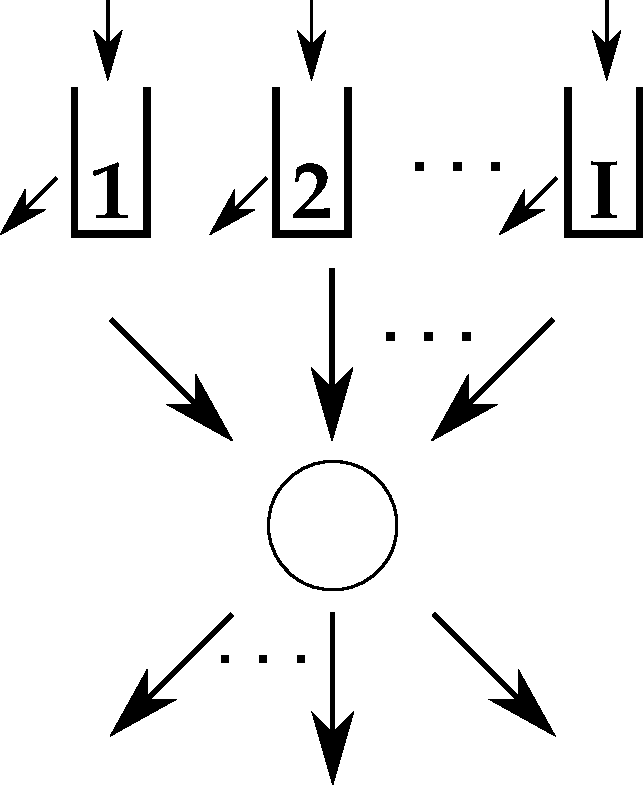
\includegraphics[width=0.4\textwidth]{pictures/p5.pdf}
  \end{center}
\end{frame}

%%%%%%%%%%%%%%%%%%%%%%%%%%%%%%%%%%%
\begin{frame}
  \frametitle{The Model}
  %\framesubtitle{The Model}
  \vfill
  \only<1->{
    \begin{tabular}{lc}
	  \begin{tabular}{l}
		\parbox{0.4\linewidth}{
	 	  \vfill		
		  \begin{itemize}[<+->]%
	 		\uncover<1->{\item \textcolor{blue}{$I$ customer classes} and \\ \textcolor{red}{$1$ server}} (processor sharing). 
			\vfill  			
  		  \item Arrivals - renewal processes.
  		  \vfill
  		  \item Service times - i.i.d. 
			\vfill  			
  		  \item Abandonments - follow exponential clock.
			\vfill	  			
  		  \item Cost - holding cost + abandonments count. 
		  \end{itemize}
		  \vfill
		}
	  \end{tabular}	
	  & \begin{tabular}{c}
	      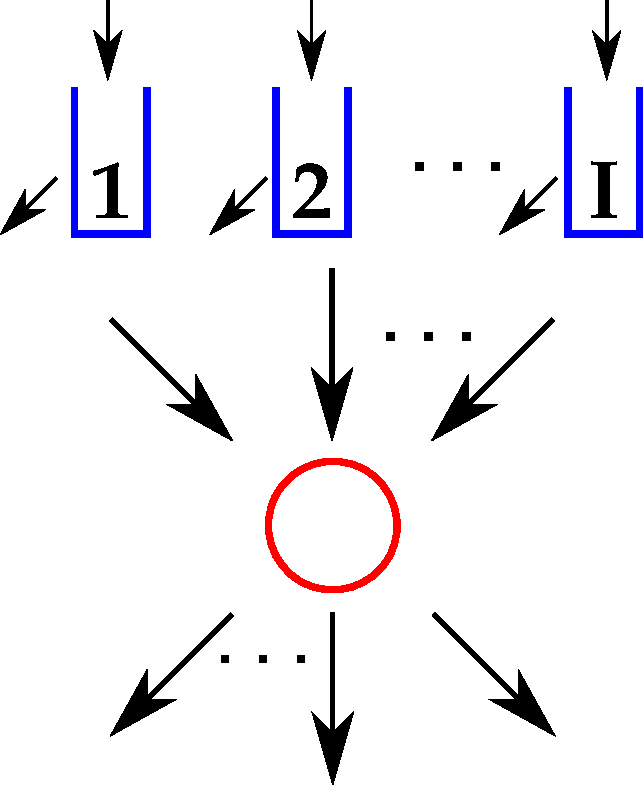
\includegraphics[width=0.4\linewidth]{pictures/p6.pdf}
	    \end{tabular} \\
    \end{tabular}
  }
  \onslide<+->{
    \vfill
        {\bf Problem: Choose who to serve next to minimize the cost}
  }
  \vfill
\end{frame}

%%%%%%%%%%%%%%%%%%%%%%%%%%%%%%%%%%%%%
\begin{frame}
  \frametitle{The Model and Control Problem}
  \framesubtitle{Mathematical Representation}

  \vfill
  \begin{itemize}[<+->]
    %\item System state process: $X(t)=(X_1(t),...,X_I(t))$
  \item $X_i(t)=$ the number of customers in the i-th class at time t
    \[
    =\underbrace{X_i(0)}_\text{initial state}+\underbrace{A_i(t)}_\text{Arrivals}-\underbrace{S_i(\int_0^t B_i(s)ds)}_\text{Departures (service)}-\underbrace{R_i(t)}_\text{Reneging}
    \]
    \vfill
  \item {\bf Cost:}
    \[
    J(B)=\mathbb{E} \Big(\int_{0}^{\infty} e^{-\alpha t} b' dR(t)\Big)=\alpha \mathbb{E} \Big(\int_{0}^{\infty} e^{-\alpha t} c' X(t)dt\Big)
    \]
      {\small where $\alpha>0$, $b_i$ reneging cost for class $i$, $c_i$ holding cost for class $i$ ($c_i=\theta_i b_i$, where $\theta_i$ is abandonment rate).} 
      \vfill
    \item {\bf Problem:} Find a control process $B(t)$ that minimizes $J(B)$.
      \vfill
    \item {\bf Not solvable analytically}.
      \vfill
    \item {\bf Approach:} Use diffusion approximation.
  \end{itemize}
  \vfill




\end{frame}
%%%%%%%%%%%%%%%%%%%%%%%%%%%%%%%%%%%%%%%%%

\begin{frame}
  \frametitle{Related Work}
  \framesubtitle{Well-Known Controls}
  
  \onslide<+->
      {
        \framebox{$c_i$ - holding cost of class $i$, $\mu_i$ - service rate, $\theta_i$ - abandonment rate }
      }
      \vfill
      \begin{itemize}[<+->]%
      \item $c\mu$-rule: Prioritize according to the $c_i\mu_i$ index \\
        \vfill
        \onslide<+->{
          $\Rightarrow$ optimal without abandonments (Smith '56) 
        }        
        \vfill
        \onslide<+->{
          $\Rightarrow$ asymptotically optimal without abandonments, including an extended (nonlinear) holding cost (special case of van Mieghem '95) 
        }
        \vfill
      \item $c\mu/\theta$-rule: Prioritize according to the $c_i\mu_i/\theta_i$ index\\
        \vfill
        \onslide<+->{
          $\Rightarrow$ asymptotically optimal with abandonments under the fluid scale (Atar Giat Shimkin 11')
        }
      \end{itemize}
      \vfill
      \onslide<+->{
        \vfill
        \bf{These results DO NOT apply in Diffusion scale.}
      }
      \vfill
\end{frame}


\begin{frame}
  \frametitle{More Related Work}
  %\framesubtitle{The Brownian Control Problem (BCP)}

  \begin{enumerate}
  \item \bibentry{GW}
  \item \bibentry{KW}
  \item \bibentry{AT}
  \item \bibentry{RubinoA09} 
  \end{enumerate}
\end{frame}



%%%%%%%%%%%%%%%%%%%%%%%%%%%%%%%%%%%%%%%%%%%%

\begin{frame}
  \frametitle{Find Asymptotically Optimal Control - Solution Steps}
  \vfill
  \begin{enumerate}[<+->]%
  \item {\bf Define BCP}: consider a sequence of systems, generated from the original system under the diffusion scale, to arrive at a Brownian Control Problem (BCP).
  %{\small The parameters are scaled as follow ($\lambda$ corresponds to the arrivals rate)\\ 
%$\frac{\lambda^n_i}{n} \to \la_i, \frac{\mu^n_i}{n} \to \mu_i,
%\theta^n_i \to \theta_i, \qquad 
%\hat{\lambda}^n_i=\frac{\lambda^n_i-n\la_i}{\sqrt{n}} \to \hat{\lambda}_i,
%\hat{\mu}^n_i=\frac{\mu^n_i-n\mu_i}{\sqrt{n}} \to \hat{\mu}_i$.
%}
	\vfill  
  \item {\bf Solve BCP}: compute the corresponding Bellman equation and deduce the control from it.\\
{\small (The Bellman equation characterize the value function)}	
	\vfill  
  \item {\bf AO}: prove this control is Asymptotically Optimal. 
  \end{enumerate}
  \vfill
\end{frame}
%%%%%%%%%%%%%%%%%%%%%%%%%%%%%%%%%%%%%%%%%%%%%



\subsection{The Brownian Control Problem (BCP)}


%\begin{frame}
%  \frametitle{The Diffusion Scaled Process}
%  \framesubtitle{The Diffusion Approximation}
%\vfill
%\onslide<+->
%{
%The number of class $i$ customers at time t in the $n$-th system \\ (under diff. scale): 
%    \begin{align*}
%    &\hat{X}_i^n(t)=\frac{X^n_i(t)}{\sqrt{n}}=\\
%    &\hat{X}_i^n(0)+\hat{W}^n_i(t)-\int_0^t \theta_i\hat{X}_i^n(s) ds+\hat{Y}_i^n(t)+e^n_i(t)
%    \end{align*}
%}
%\vfill
%\only<2->
%{   
%where
%  \begin{enumerate}[<+->]%
%  \item $\hat{W}^n_i(t)=y^n_it+\hat{A}^n_i(t)-\hat{D}^n_i(t)$ centered arrival and departure processes, converge by FCLT to a BM  
%  \vfill
%  \item $\hat{Y}_i^n(t)$ is the control.
%  \end{enumerate}
%}
%\vfill
%\end{frame}


%\begin{frame}

%\subsubsection{The Brownian Control Problem (BCP)}

\begin{frame}
  \frametitle{Step $1$ - Defne BCP}
  %\framesubtitle{The Brownian Control Problem (BCP)}

  \vfill
  \begin{itemize}[<+->]
  \item $X_t=x+\underbrace{W_t}_\text{BM}-\int_0^t \underbrace{\Theta}_\text{$\diag(\theta)$} X_s ds +\underbrace{Y_t}_\text{Control}\in \mathbb{R}^I_{+}$
    \vfill
  \item {\bf Heavy traffic condition:} $\sum_{i=1}^I \lambda_i/\mu_i=1$\\
    {\small $\lambda$, $\mu$ are first order approximations for the arrival rate and service rate}
    \vfill
  \item {\bf Goal:} To minimize the cost function 
    \begin{equation*}\label{cost}
      J(x,Y)=\mathbb{E} \Big(\int_{0}^{\infty} e^{-\alpha t} \underbrace{c'}_\text{holding cost} X_t dt\Big).
    \end{equation*}
    for $Y$ being admissible

  \end{itemize}
  \vfill



\end{frame}
%%%%%%%%%%%%%%%%%%%%%%%%%%%%%%%%%%%%%%%%%%%%

\begin{frame}
  \frametitle{Step $1$ - Define BCP}
    \framesubtitle{Admissible Control}
    \only<1>{
    \begin{definition}
      {\it admissible control system} with initial condition $x \in \mathbbm{R}^I_+$ is a tuple
      $(\bar\Sig,W_t, Y_t, X_t)$,
      where $\bar\Sig=(\bar{\Om},\bar{\mathcal{F}}, \{\bar{\mathcal{F}}_t\}, \bar{P})$ is a filtered
      probability space, $\{W_t\}$ is an $I$-dimensional $\bar\calF_t$-adapted $(y,\sig)$-BM,
      the processes $\{X_t\}$ and $\{Y_t\}$ have sample paths in $\D_{\R^I}(\R_+)$ and are
      $\bar\calF_t$-adapted, and the following hold:
      \begin{enumerate}
      \item[i.] For all $t,s\geq 0$, $W_{t+s}-W_t$ is independent of $\bar\calF_t$ under $\bar{P}$,

      \item[ii.] $X_t$ satisfies $X_t\in\R_+^I$
        for all $t$ $\bar P$-a.s.,

      \item[iii.] The process $m' Y$, where $m=(1/\mu_1,...,1/\mu_I)$, is non-negative and non-decreasing.

      \end{enumerate}
    \end{definition}
    
  }
  \only<2->{
    \begin{definition}
      \textcolor{gray}{{\it admissible control system} with initial condition $x \in \mathbbm{R}^I_+$ is a tuple
      $(\bar\Sig,W_t, Y_t, X_t)$,
      where $\bar\Sig=(\bar{\Om},\bar{\mathcal{F}}, \{\bar{\mathcal{F}}_t\}, \bar{P})$ is a filtered
      probability space, $\{W_t\}$ is an $I$-dimensional $\bar\calF_t$-adapted $(y,\sig)$-BM,
      the processes $\{X_t\}$ and $\{Y_t\}$ have sample paths in $\D_{\R^I}(\R_+)$ and are
      $\bar\calF_t$-adapted, and the following hold:}
      \begin{enumerate}
      \item[i.] \textcolor{gray}{For all $t,s\geq 0$, $W_{t+s}-W_t$ is independent of $\bar\calF_t$ under $\bar{P}$,}

      \item[ii.] \textcolor{gray}{$X_t$ satisfies $X_t\in\R_+^I$
        for all $t$ $\bar P$-a.s.,}

      \item[iii.] \textcolor{black}{The process $m' Y$, where $m=(1/\mu_1,...,1/\mu_I)$, is non-negative and non-decreasing.}

      \end{enumerate}
    \end{definition}
    
  }
  \vfill
  \only<3->{
  \begin{itemize}
  \item $\mathcal{A}(x)$ the set of all admissible control systems with initial condition $x \in \mathbbm{R}^I_+$.
  \vfill
 \item {\bf The value function}
    \begin{equation*}\label{valuef}
      V(x)=\inf_{\mathcal{A}(x)} J(x,Y),\qquad x\in\mathbbm{R}_{+}^I.
    \end{equation*}
  \end{itemize}
    
  \vfill
}
\end{frame}
%%%%%%%%%%%%%%%%%%%%%%%%%%%%%%%%%%%%%%%%%%%%
\subsection{Solving the BCP}

\subsubsection{The Bellman Equation}
\begin{frame}
  \frametitle{Step $2$- Solve BCP}
  \framesubtitle{The Bellman Equation}
  \vfill
  $I$-th dimensional equation.
  \vfill
  \pause
  \begin{itemize}[<+->]
  \item  {\bf Problem}: hard to solve.
    \vfill
  \item {\bf Solution:} Reduction to $1$-dimension - Reduced Brownian Control Problem (RBCP).\\
    Often occurs and is called State Space Collapse property (SSC)
  \end{itemize}
  \onslide<+->{
  \vfill
    The two problems are equivalent 
  }
  \vfill

\end{frame}




\begin{frame}
  \frametitle{Step $2$- Solve BCP}
  \framesubtitle{The RBCP}

  \vfill
  \begin{itemize}[<+->]
  \item Projection to the workload vector $m=(1/\mu_1,...,1/\mu_I)$. 
    \vfill
  \item {\bf Workload process} 
    \[
    \tilde {X}_t=m' X(t)=\tilde{x}+\tilde{W}_t-\int_0^t \theta' U_s \tilde{X}_s ds+\tilde{Y}_t.
    \]

    \vfill
  \item {\bf Control:} the pair $(U,\tilde Y)$.
    \begin{itemize}[<+->]%
    \item $\tilde Y=m' Y$ 
    \item $U$ is an I-dimensional process corresponds to the division of the workload between the classes $\rightarrow U_i$ is the fraction of workload dedicated to class $i$.
    \end{itemize}
    \vfill
  \item {\bf Cost:}
    \[
    \tilde{J}(\tilde{x},(U,\tilde{Y}))
    =\mathbb{E} \Big(\int_{0}^{\infty} e^{-\alpha t} q'U_t\tilde{X}_{t}dt\Big).
    \]
  \end{itemize}
  \vfill
  
\end{frame}
%%%%%%%%%%%%%%%%%%%%%%%%%%%%%%%%%%%%%%%%%%%


\begin{frame}
  \frametitle{Step $2$- Solve BCP}
  \framesubtitle{Admissible Control, RBCP}
  \only<1>{
    \begin{definition}\label{adm1-dDCP}
      An {\it admissible control system} with initial condition $\tilde{x} \in \R_+$ is a tuple
      $(\tilde\Sig,\tilde W, {U}, \tilde{Y}, \tilde{X})$,
      where $\tilde\Sig=(\tilde{\Om},\tilde{\mathcal{F}}, \{\tilde{\mathcal{F}}_t\}, \tilde{P})$
      is a filtered probability space, $\{\tilde{W}_t\}$ is a $1$-dimensional $\tilde\calF_t$-adapted
      $(\tilde y,\tilde\sig)$-BM,
      and the processes $\{{U}_t\}$, $\{\tilde{Y}_t\}$, $\{\tilde X_t\}$ have sample paths in
      $\D_{\calS_1}(\R_+)$, $\D_{\R^I}(\R_+)$ and $\D_\R(\R_+)$, resp., are $\tilde\calF_t$-adapted
      and the following hold:
      \begin{enumerate}%
      \item[i.] For all $t,s\geq 0$, $\tilde{W}_{t+s}-\tilde{W}_t$ is independent
        of $\tilde\calF_t$ under $\tilde{P}$,

      \item[ii.] $\tilde X_t$ satisfies $\tilde X_t\ge0$
        for all $t$ $\tilde{P}$-a.s.,

      \item[iii.] The process $\tilde Y$ is non-negative and non-decreasing.

      \end{enumerate}
    \end{definition}
  }
  \only<2->{
    \begin{definition}\label{adm1-dDCP}
    	\textcolor{gray}{
      An {\it admissible control system} with initial condition $\tilde{x} \in \R_+$ is a tuple
      $(\tilde\Sig,\tilde W, {U}, \tilde{Y}, \tilde{X})$,
      where $\tilde\Sig=(\tilde{\Om},\tilde{\mathcal{F}}, \{\tilde{\mathcal{F}}_t\}, \tilde{P})$
      is a filtered probability space, $\{\tilde{W}_t\}$ is a $1$-dimensional $\tilde\calF_t$-adapted
      $(\tilde y,\tilde\sig)$-BM,
      and the processes $\{{U}_t\}$, $\{\tilde{Y}_t\}$, $\{\tilde X_t\}$ have sample paths in
      $\D_{\calS_1}(\R_+)$, $\D_{\R^I}(\R_+)$ and $\D_\R(\R_+)$, resp., are $\tilde\calF_t$-adapted
      and the following hold:}
      \begin{enumerate}%
      \item[i.] \textcolor{gray}{For all $t,s\geq 0$, $\tilde{W}_{t+s}-\tilde{W}_t$ is independent
        of $\tilde\calF_t$ under $\tilde{P}$,}

      \item[ii.] \textcolor{gray}{$\tilde X_t$ satisfies $\tilde X_t\ge0$
        for all $t$ $\tilde{P}$-a.s.,}

      \item[iii.] The process $\tilde Y$ is non-negative and non-decreasing.

      \end{enumerate}
    \end{definition}
  }
  \vfill
  \only<3->{
  \begin{itemize}
   \item $\tilde{\mathcal{A}}(\tilde{x})$ the set of all the admissible controls for the
    initial condition $\tilde x$.
  \vfill
  \item {\bf Value function:}
    \[
    \tilde{V}(\tilde{x})=\inf_{({U},\tilde{Y}) \in \tilde{\mathcal{A}}(\tilde{x})} \tilde{J}(\tilde{x},({U},\tilde{Y})), \qquad \tilde x\in\R_+.
    \]
 \end{itemize}
 \vfill
 }
\end{frame}



\begin{frame}
\frametitle{Step $2$- Solve BCP}
  \framesubtitle{The Bellman Equation}
  % \frametitle{Step $2$- Solve BCP}
  \onslide<+->{
    
    \begin{align*}
      \begin{cases}
        &  -\frac{\tilde\sigma^2}{2}\frac{d^2v}{dx^2}-\tilde{y}\frac{dv}{dx}
        +x F\Big(\frac{dv}{dx}\Big)+\alpha v=0,\qquad 0<x<\iy,\\
        &\frac{dv}{dx}(0)=0,\qquad |v(x)|\le C(1+x)^C, \qquad x\in[0,\iy).
      \end{cases}
    \end{align*}       
        }
        \vfill
        \only<2->{  
          where
          \begin{itemize}[<+->]%
          \item $F(y)=\max_u g(u,y)$, $u$ corresponds to the original control.
            \vfill
          \item $\tilde y$, $\tilde\sigma$ - system parameters.
            \vfill
          \item The Bellman equation admits a unique classical solution - the value function $\tilde{V}$ .
            \vfill
          \item The optimal control is deduced from finding the maximum in $F(y)=\max_u g(u,y)$.
            \vfill
          \item Can be solved numerically (equation in one variable).                  
          \end{itemize} 
          \vfill
        }
\end{frame}

\begin{frame}
\frametitle{Step $2$- Solve BCP}
  \framesubtitle{Optimal Control Derivation}
  

  \vfill
  \begin{itemize}[<+->]
  \item $g(u,y)=\theta \cdotp u y - q \cdotp u$
    \vfill
  \item $u\in \{a\in \mathbb{R}_{+}^I| \sum_i a_i=1 \}$
  \end{itemize}
  \vfill
  \onslide<+->{
    $$
    \Rightarrow \text{The maximal solution is one of the extreme points:}$$
    \center $u\in \{e_1,...,e_I\}$- the standard basis
  }  
  \vfill
  \onslide<+->{
    \[
    \Rightarrow F(y)=\max_u g(u,y)=\max_i\ph_i(y), \qquad \ph_i(y)=\theta_iy-c_i\mu_i,\quad y\in\R_+ 
    \]
  }
  \vfill 
\end{frame}

\subsubsection{Optimal Control Derivation}
\begin{frame}
  \frametitle{Step $2$- Solve BCP}
  \framesubtitle{Optimal Control Derivation - Example}

  \begin{figure}\label{fig1}
    \begin{center}
      %\includegraphics[width=30em, height=15em]
      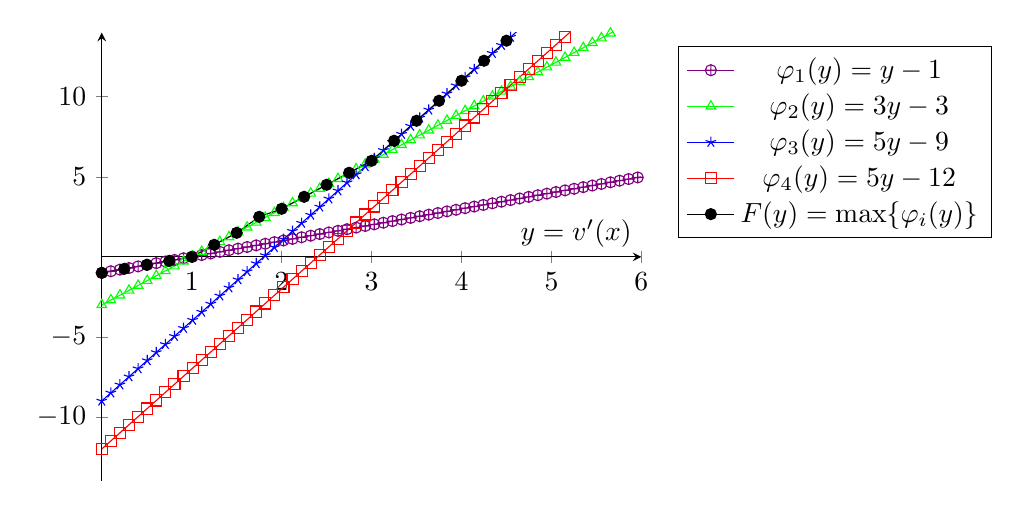
\begin{tikzpicture}
        \begin{axis}[
            axis lines = middle,
            xlabel = {$y=v'(x)$},
            legend style={at={(1.65,0.97)},
              anchor=north east},
            xmin=0, xmax=6,
            ymin=-14, ymax=14,
          ]
          \centering
          \addplot [
            domain=0:10,
            samples=100,
            color=violet,
            mark=oplus,
          ]
                   {x-1};
                   \addlegendentry{$\varphi_1(y)=y-1$}

                   \addplot [
                     domain=0:10,
                     samples=100,
                     color=green,
                     mark=triangle
                   ]
                            {(3*x -3};
                            \addlegendentry{$\varphi_2(y)=3y -3$}


                            \addplot [
                              domain=0:10,
                              samples=100,
                              color=blue,
                              mark=star,
                            ]
                                     { 5*x -9};
                                     \addlegendentry{$\varphi_3(y)=5y -9$}


                                     \addplot [
                                       domain=0:10,
                                       samples=100,
                                       color=red,
                                       mark=square,
                                     ]
                                              {5*x - 12};
                                              \addlegendentry{$\varphi_4(y)=5y - 12$}


                                              \addplot [
                                                color=black,
                                                mark=otimes*,
                                              ]
                                              coordinates {
                                                (0,-1) (0.25,-0.75) (0.5,-0.5) (0.75,-0.25) (1,0) (1.25,0.75) (1.5,1.5) (1.75,2.5) (2,3)
                                                (2.25,3.75) (2.5,4.5) (2.75,5.25) (3,6) (3.25,7.25) (3.5,8.5) (3.75,9.75) (4,11)
                                                (4.25,12.25) (4.5, 13.5) };
                                              \addlegendentry{$F(y)=\max \{\varphi_i(y)\}$}


        \end{axis}
      \end{tikzpicture}


    \end{center}
  \end{figure}

  %$3$ different intervals for $v'$: $[0,1),[1,3),[3,\infty)$.\\
  %On each interval the control process satisfy: $U=e_i$ $\rightarrow$ all the workload remains in the $i$-th class.\\
  %The intervals for $v'$ correspond to interval for $\tilde{X}$ - $[0,w_1),[w_1,w_2),[w_2,\infty)$ ($v$ is nondecreasing and convex) 

\end{frame}


\begin{frame}
  \frametitle{Step $2$- Solve BCP}
  \framesubtitle{Optimal Control Derivation - Example}
  
  \begin{center}
    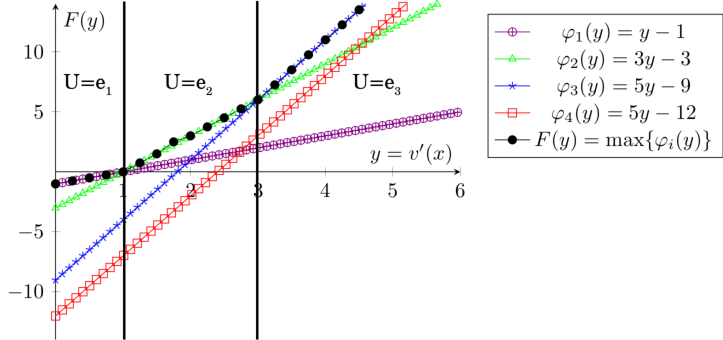
\includegraphics[width=0.9\textwidth]{pictures/graphWithLines.pdf}
  \end{center}

  \vfill
  \onslide<+->{
    \begin{itemize}[<+->]
    \item $3$ different intervals for $v'$: $[0,1),[1,3),[3,\infty)$
          \vfill
        \item On each interval the control process satisfy $U=e_i$\\
          \vfill
          \onslide<+->{
            $\rightarrow$ all the workload remains in the $i$-th class.}
    \end{itemize}
        }
        \vfill

\end{frame}

\begin{frame}
  \frametitle{Step $2$- Solve BCP}
  \framesubtitle{Optimal Control Derivation - Example}
  
  \begin{center}
    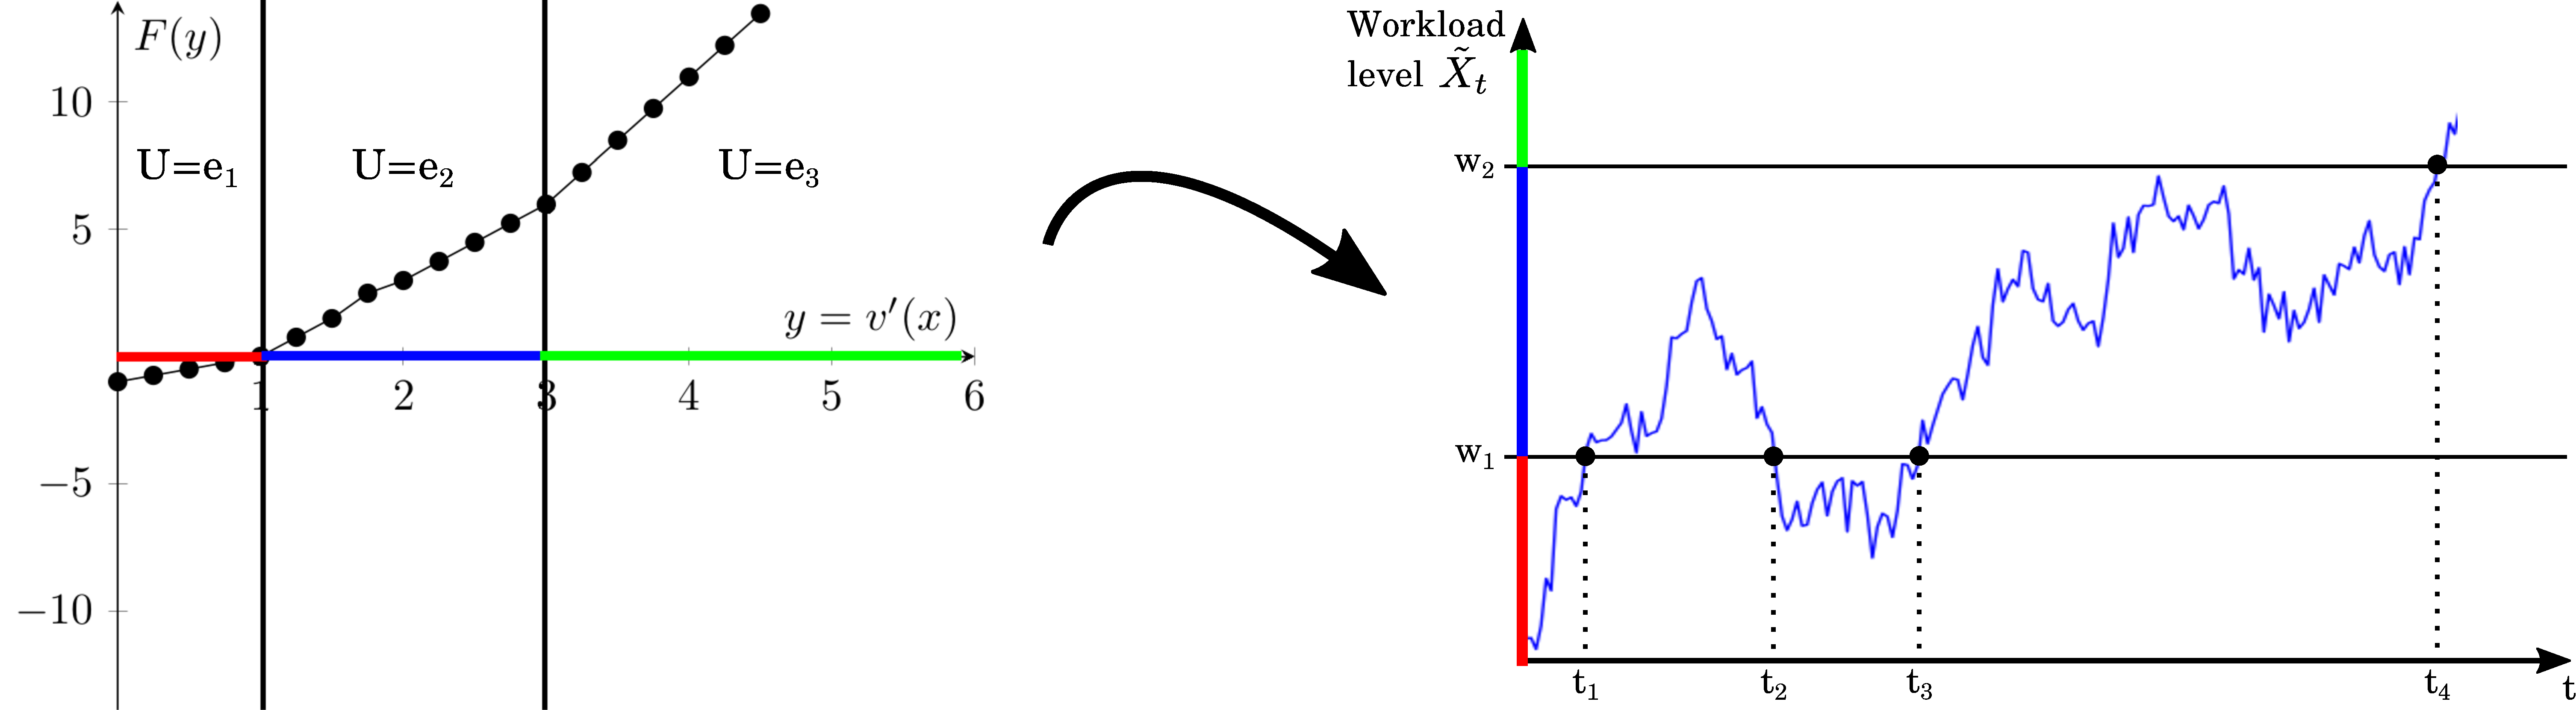
\includegraphics[width=0.9\textwidth]{pictures/p20WithAddition.pdf}
  \end{center}

  \vfill
  \begin{itemize}[<+->]
  \item $v$ is nondecreasing and convex 
    \vfill
  \item The intervals for $v'$ correspond to interval for $\tilde{X}$ - $[0,w_1),[w_1,w_2),[w_2,\infty)$
  \end{itemize}
  \vfill

\end{frame}

\begin{frame}
  \frametitle{Step $2$- Solve BCP}
  \framesubtitle{Optimal Control Derivation - Example}
  
  \begin{center}
    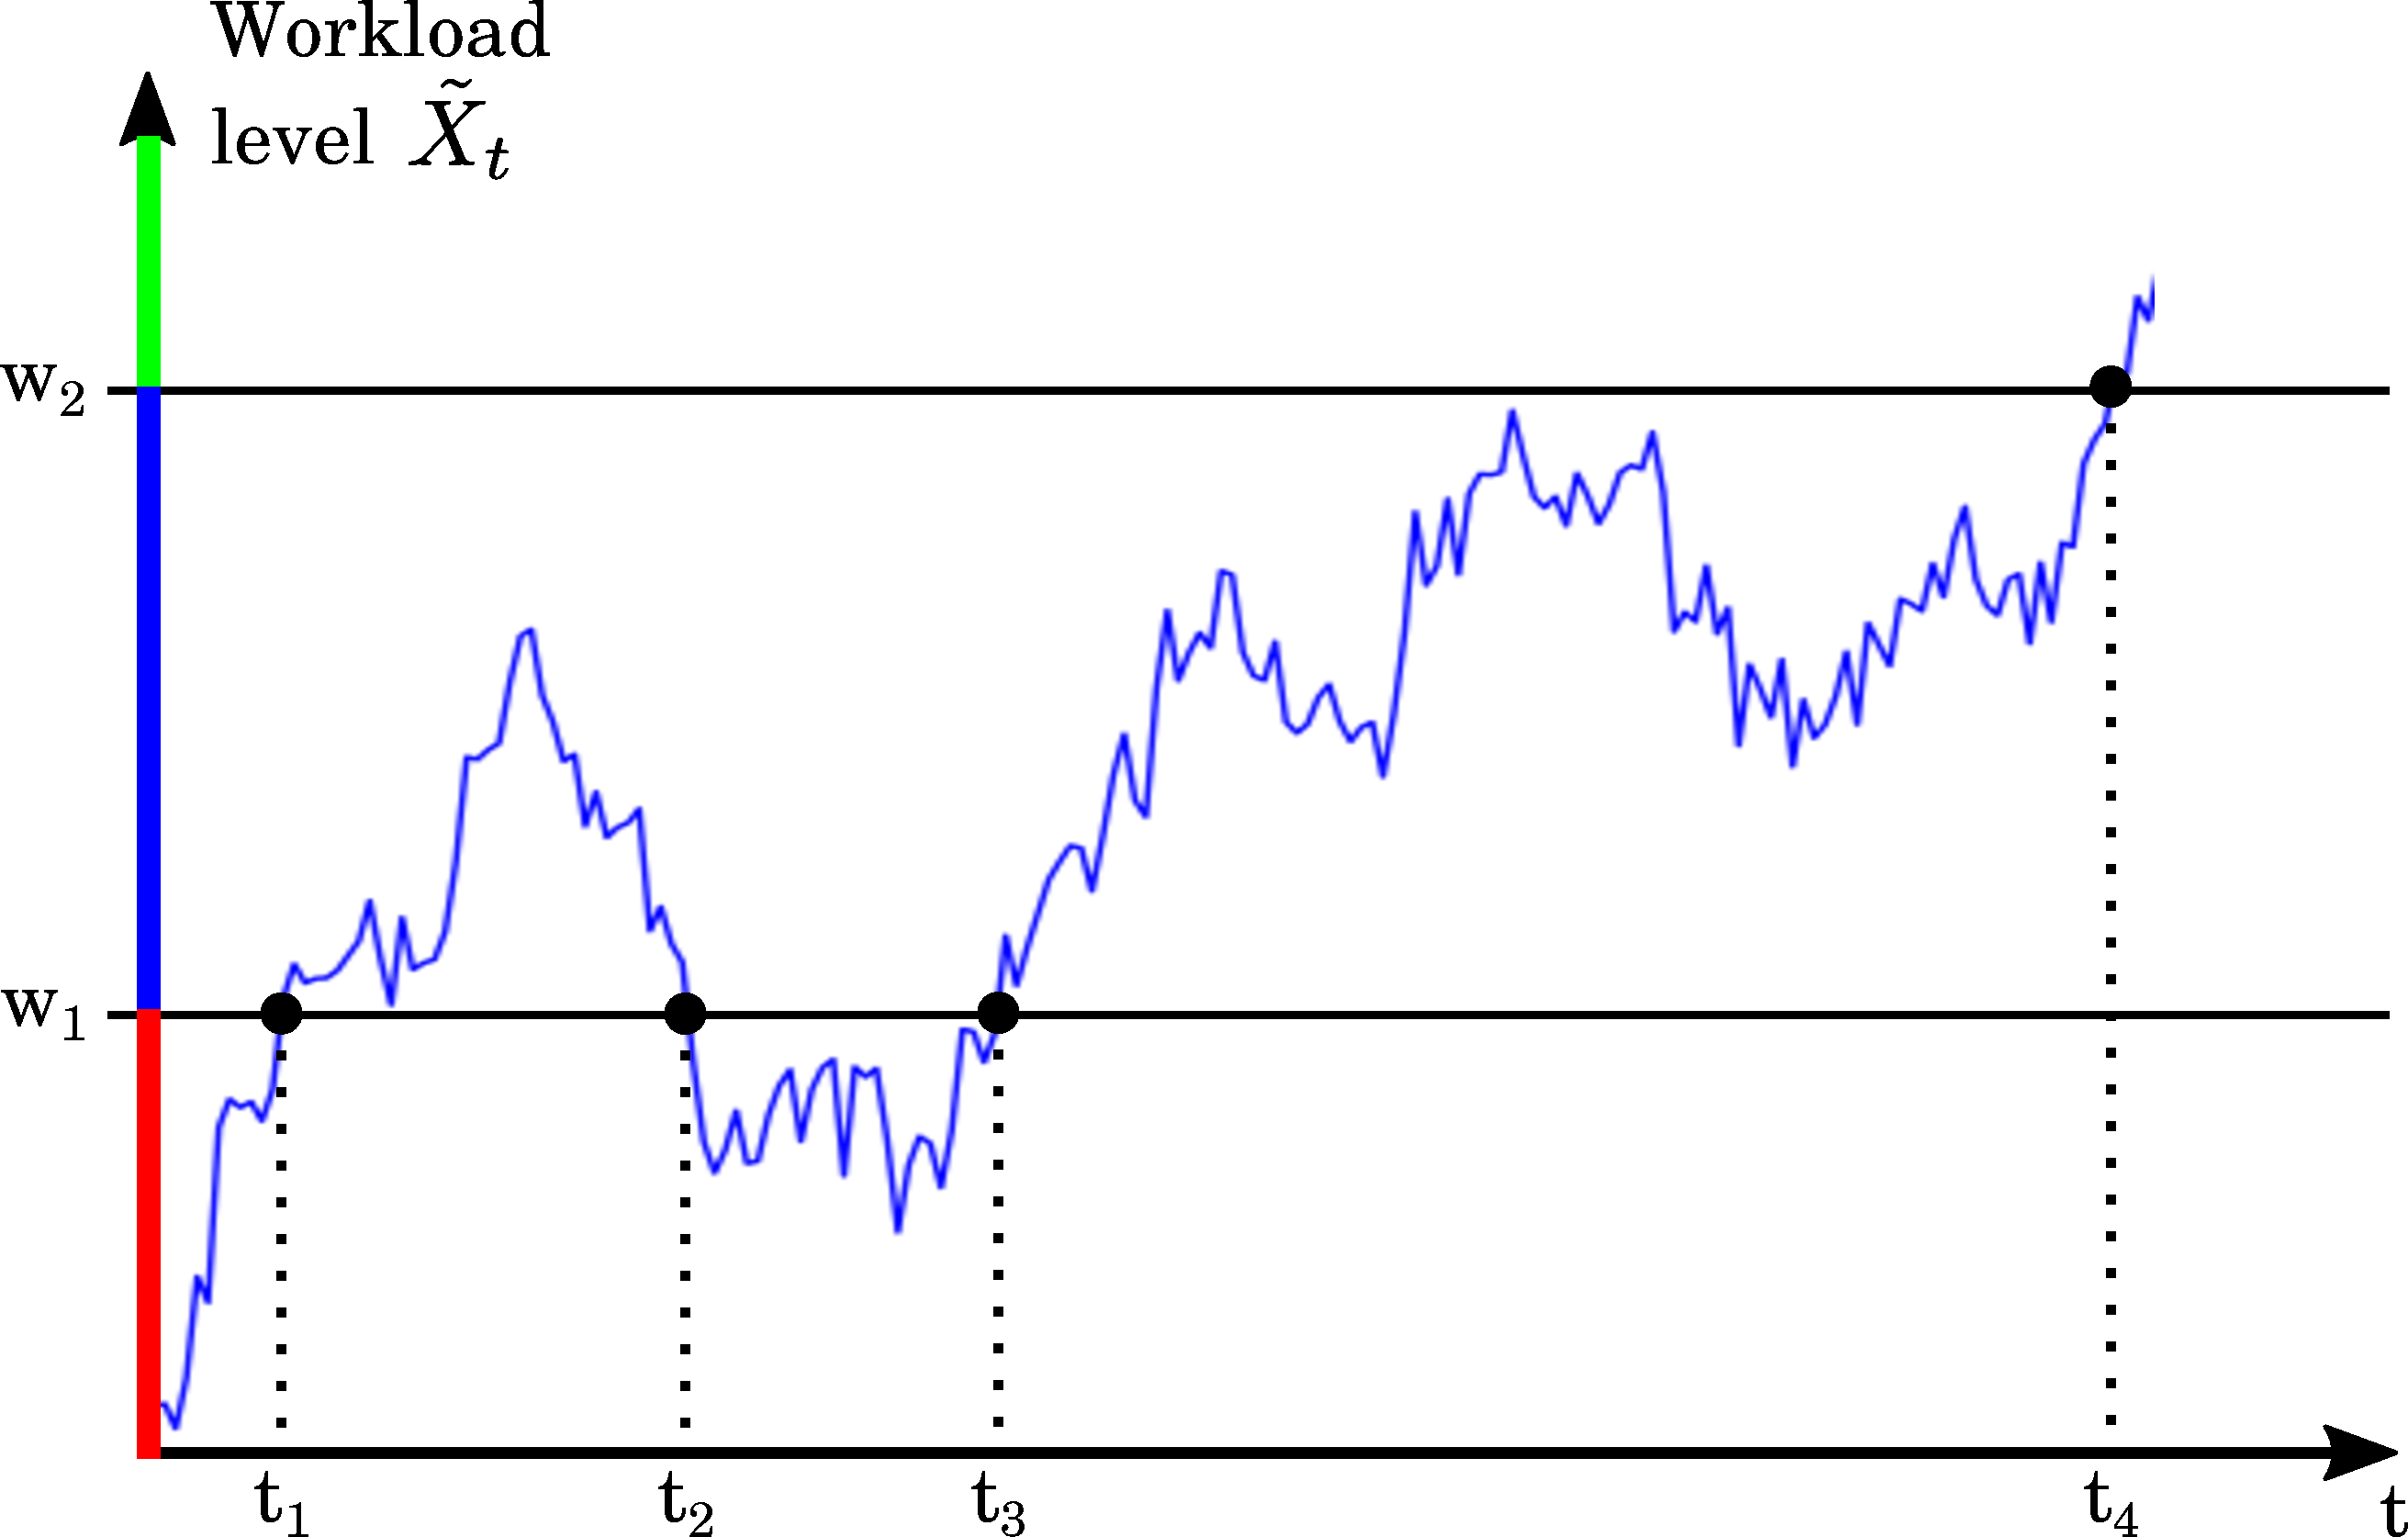
\includegraphics[width=0.9\textwidth]{pictures/p20.pdf}
  \end{center}

  \vfill  
  \onslide<+->{
    {\bf Ex.} Below $w_1$ ($[0,t_1)$, $[t_2,t_3)$,...): $U=e_1$ $\rightarrow$ least priority to class $1$.
      }
\end{frame}



\begin{frame}
\frametitle{Step $2$- Solve BCP}
  \framesubtitle{The Optimal Control $B^{n,*}$ - Definition}
  
  \vfill  
  \onslide<+->{
    $\calK$ is a minimal subset of $\calI$ such that
    $\max_{k\in\calK}\ph_k(y)=\max_{i\in\calI}\ph_i(y)$  
  }
  \vfill
  \only<2->{
    Assumptions: 
    \begin{enumerate}[<+->]%
    \item $c_1\mu_1\leq c_2\mu_2\leq \cdots\leq c_K\mu_K$.
      \vfill
    \item $\{L_k\}_{k\in\calK}$ a partition of $[0,\iy)$. 
    \end{enumerate}
    \vfill
	}
	  \onslide<+->{
        \vfill
            {\bf The optimal policy:}
            \vfill  
            \begin{enumerate}[<+->]%
            \item Non-interruptible, non-idling policy that allows no processor sharing.
              \vfill
            \item At time $t$, the server becomes available and some of the buffers are non-empty,
              the current value of the scaled workload $\tilde X^n_t$ is computed and the {\bf least priority class} $k$
              is set to be the unique $i$ for which $\tilde X^n_t\in L_i$.
              \vfill
            \item The customer to be served is then picked according to the ordering
              \[
              (k+1,k+2,\ldots,I,1,2,\ldots,k).
              \]

            \end{enumerate}
            \vfill
      }
\end{frame}

\begin{frame}
  \frametitle{Step $2$- Solve BCP}
  \framesubtitle{The Optimal Control - Example}
  
  \begin{center}
    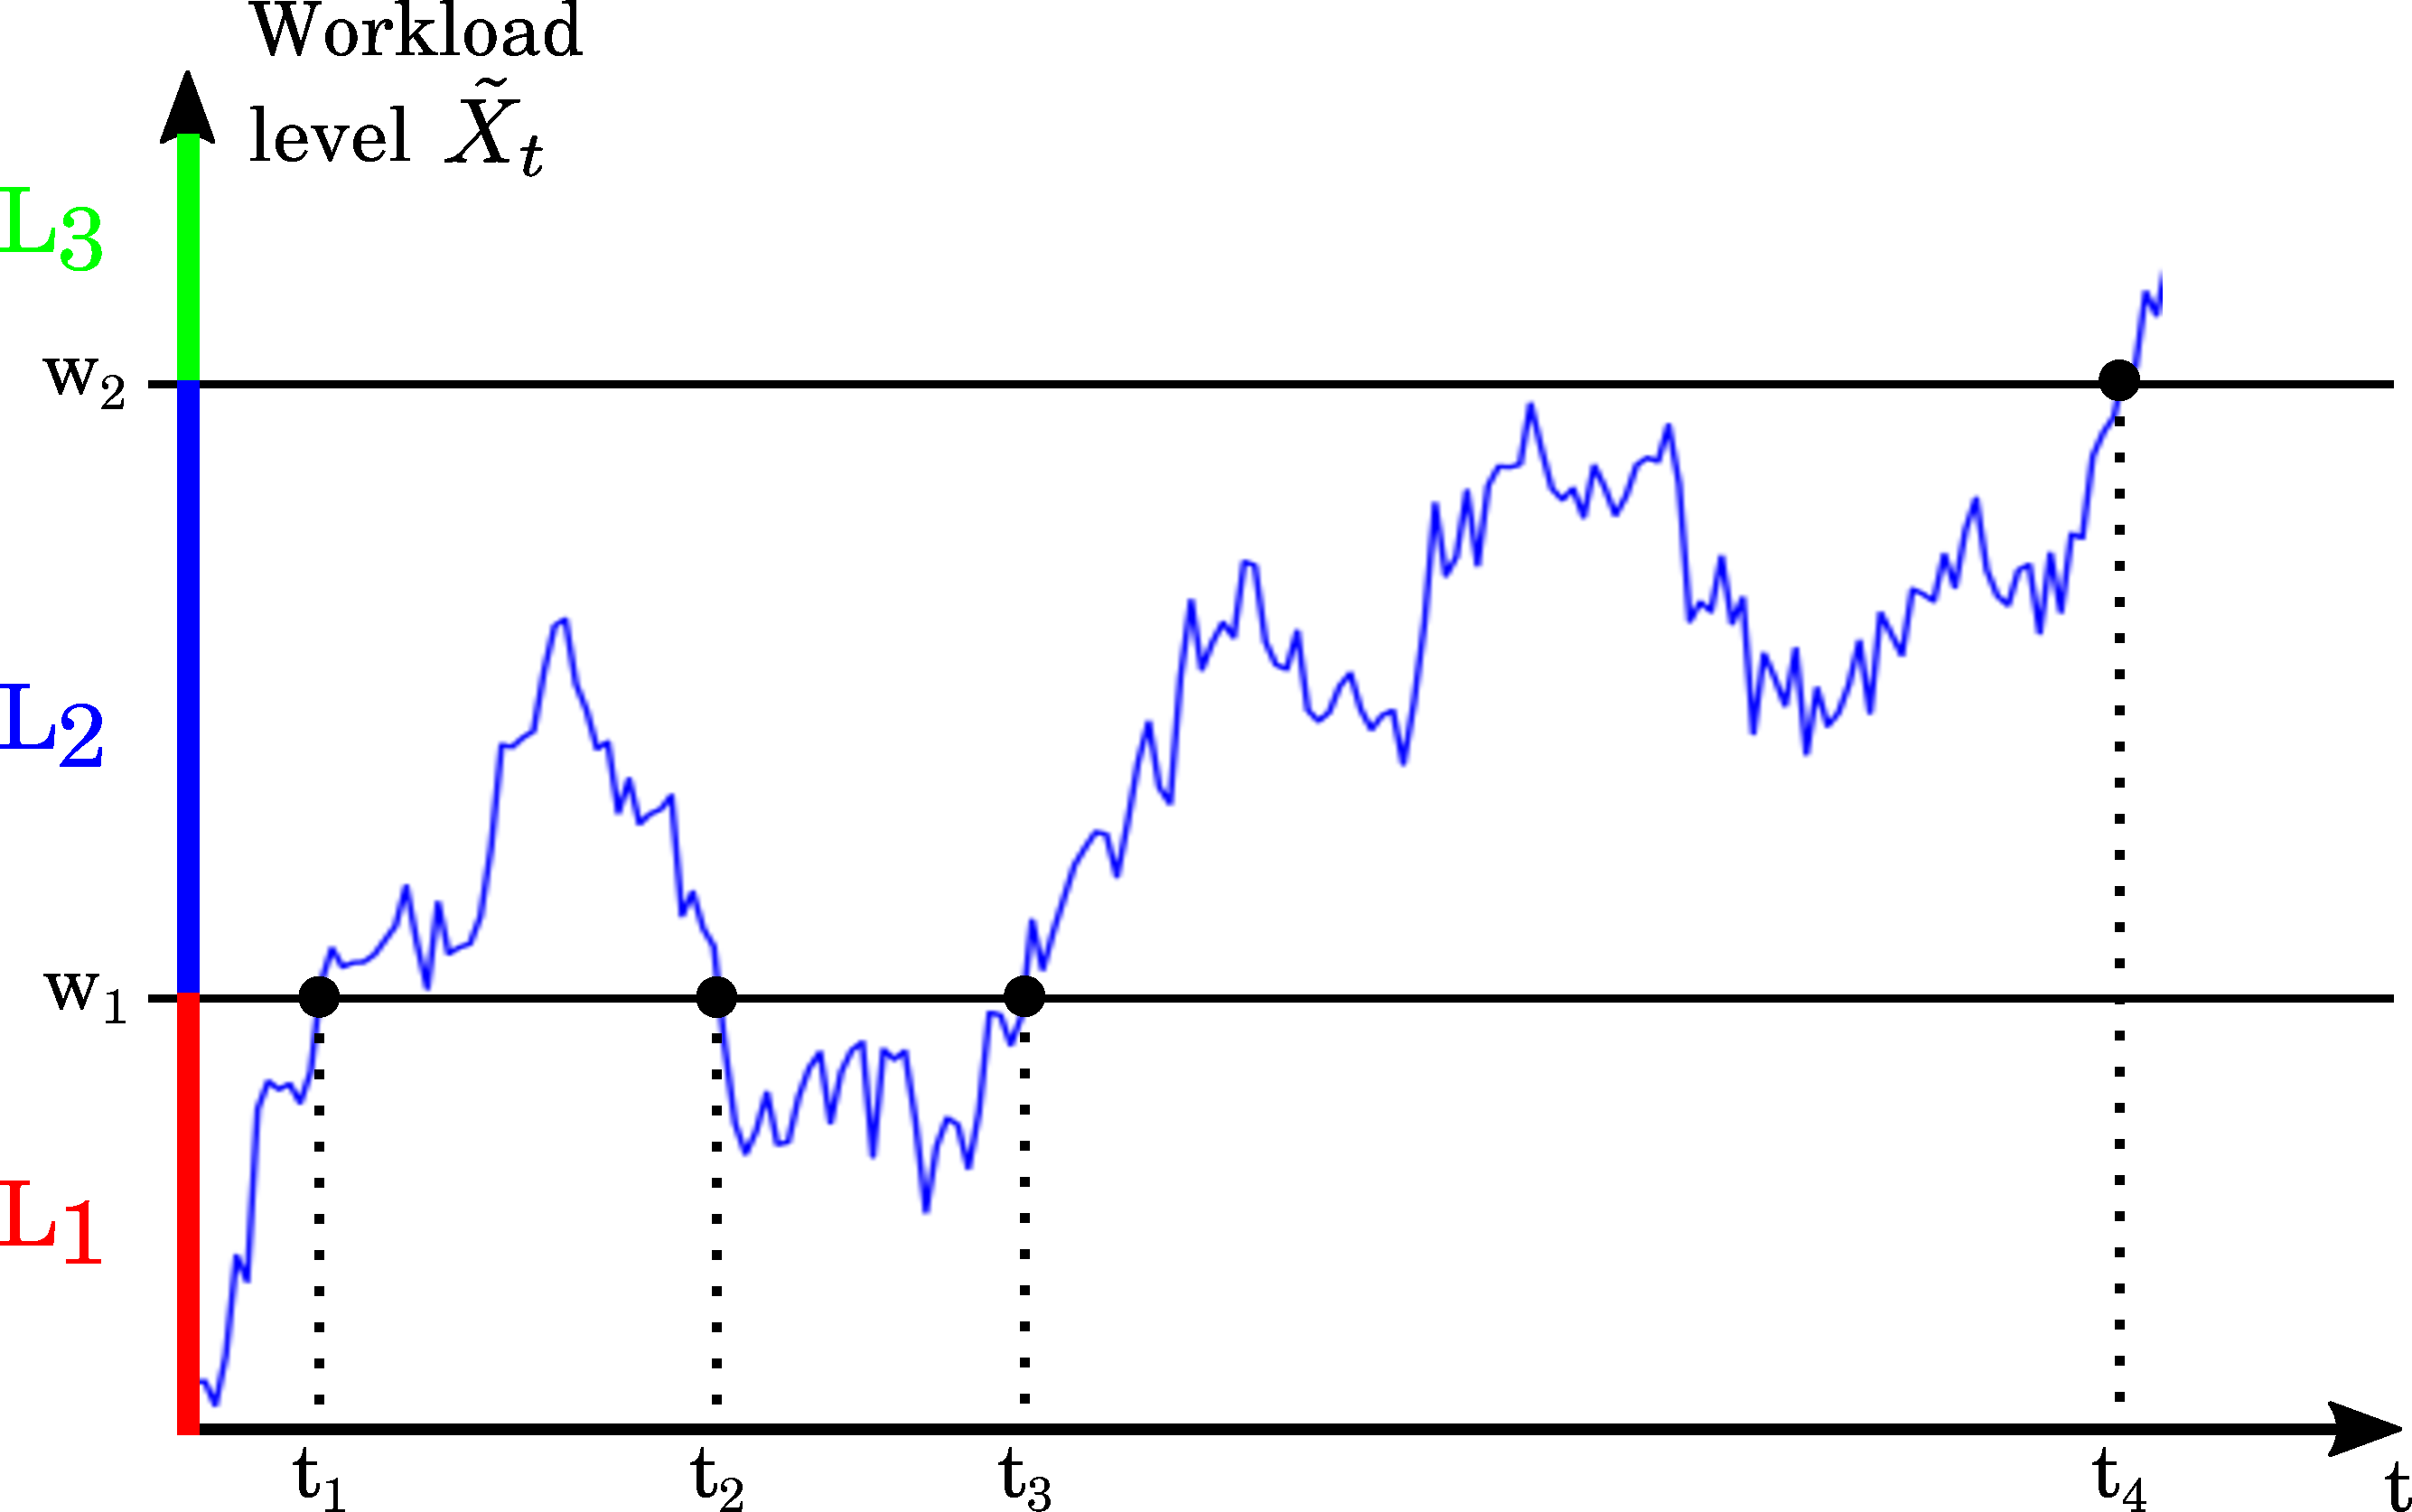
\includegraphics[width=0.9\textwidth]{pictures/p20c.pdf}
  \end{center}

\vfill
\mbox{$\calI=\{1,2,3,4\}$, $\calK=\{1,2,3\}$, $c_1\mu_1\leq c_2\mu_2\leq c_3\mu_3$}
\vfill
  
\end{frame}

\begin{frame}
  \frametitle{Step $2$- Solve BCP}
  \framesubtitle{The Optimal Control}

  \vfill
  \begin{itemize}[<+->]
  \item Dynamic index rule. {\bf Not static index rule as $c\mu$ or $c\mu/\theta$}.
    \vfill
  \item When workload is \textcolor{red}{low} the server gives least priority to class with lowest $c\mu$ index.
    \vfill
  \item When workload is \textcolor{green}{high} the server gives least priority to class with highest $\theta$ index.
  \end{itemize}
  \vfill



\end{frame}


%%%%%%%%%%%%%%%%%%%%%%%%%%%%%%%%%%%%%%%%%%

\subsection{Main Result}
\begin{frame}
  \frametitle{Step $3$ - AO}
  \framesubtitle{Main Result}

  
  \begin{theorem}
    \label{th1}
    Let $v$ denote the solution of the Bellman equation. Then\\
    $i$.The limit value is determined by the function $v$. In particular,
    \[
    \lim_{n\to\iy}\hat V^n= v(m'x_0).
    \]
    ii. The control process $B^{n,*}$ described above is AO, that is,
    \[
    \lim_{n\to\iy}\hat J^n(B^{n,*})= v(m'x_0).
    \]
  \end{theorem}

\end{frame}

%%%%%%%%%%%%%%%%%%%%%%%%%%%%%%%%%%%%%%%%%%%%%%%%%%%



%%%%%%%%%%%%%%%%%%%%%%%%%%%%%%%%%%%%%%%%%%

\begin{frame}
  \frametitle{Step $3$ - AO}
  \framesubtitle{Main Result - Proof Steps}

  \vfill
  \onslide<+->{
    Two parts:
  }
  \vfill 
  \begin{enumerate}[<+->]%
  \item {\bf Lower bound:}\\
    For any sequence of admissible controls
    \[
    \liminf_{n \to \infty} \hat{J}^n(B^n)\ge v(m'x_0).
    \]
    \vfill
  \item {\bf Upper bound:}\\
    Under the control process $B^{n,*}$ described earlier
    \[
    \limsup_{n \to \infty} \hat{J}^n(B^{n,*})\le v(m'x_0).
    \]
    
  \end{enumerate}
  \vfill  

\end{frame}
%%%%%%%%%%%%%%%%%%%%%%%%%%%%%%%%%%%%%%%%%%%%%%%%%%%

\begin{frame}
\frametitle{Step $3$ - AO}
   \framesubtitle{Why The Process $X$ is Discussions?}
  %\framesubtitle{The Brownian Control Problem (BCP)}
  \vfill
  \onslide<+->{
    \begin{center}
      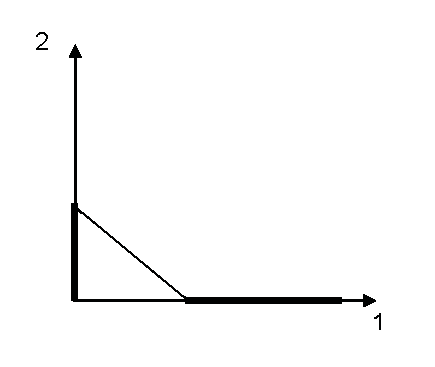
\includegraphics[width=0.4\textwidth]{pictures/fig-de-3-eps-converted-to.pdf}
      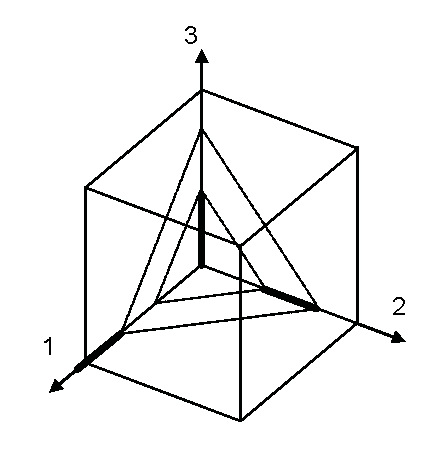
\includegraphics[width=0.4\textwidth]{pictures/fig-de-4-eps-converted-to.pdf}
    \end{center}
  }
  %\vfill
  %\begin{itemize}[<+->]
  %\item The process $\tilde{X}$ has $K$ discontinuity points $w_1,...,w_K$
  %\vfill
  %\item At each interval $[w_i,w_{i+1})$ the policy is fixed and gives least priority to class $i$
  %\end{itemize}
  %\vfill
\end{frame}

%%%%%%%%%%%%%%%%%%%%%%%%%%%%%%%%%%%%%%%%%%%
\begin{frame}
\frametitle{Step $3$ - AO}
  \framesubtitle{Main Result - Proof of the Upper Bound}
  %\framesubtitle{The Brownian Control Problem (BCP)}

  \vfill
  \begin{itemize}[<+->]
  \item {\bf Problem:} The process $X$ is discontinuous with $K-1$ discontinuity points $w_1,...,w_{K-1}$.
    \vfill
  \item {\bf Solution:}
    \begin{enumerate}[<+->]%  
    \item Show that in the interior of each interval $[w_i,w_{i+1})$ where the policy is fixed and gives least priority to class $i$, all the other classes (not the i-th class) empties. State Space Collapse property (SSC).
      \vfill
    \item  Show that the time spent around the discontinuity points $w_i$ is small $\rightarrow$ can be neglected. 

    \end{enumerate}
  \end{itemize}
  \vfill
\end{frame}

%%%%%%%%%%%%%%%%%%%%%%%%%%%%%%%%%%%%%%%%%%%%%%%%%%%%%%%%%%%%%%%%%%%%%%%%%%%%%%%%%



%%%%%%%%%%%%%%%%%%%%%%%%%%%%%%%%%%%%%%%%%%%%%%%%%%%%%%%%%%%%%%%%%%%%%%%%%%%%%%%%%

\section{The $G/G/1$ Queue with Retrials}

\subsection{The Model}
%%%%%%%%%%%%%%%%%%%%%%%%%%%%%%%%%%%%%%%%%%%%%%%%%%%%%%%%%%%%%%%%%%%%%%%%%%

%% \begin{frame}
%%   \frametitle{The $G/G/1$ Queue with Retrials}
%%   \framesubtitle{The queue}

%%   Enter picture of a router. Something visual and pretty.
%% \end{frame}

\begin{frame}
  \frametitle{The $G/G/1$ Queue with Retrials}
  \framesubtitle{The Model}
  \begin{center}
    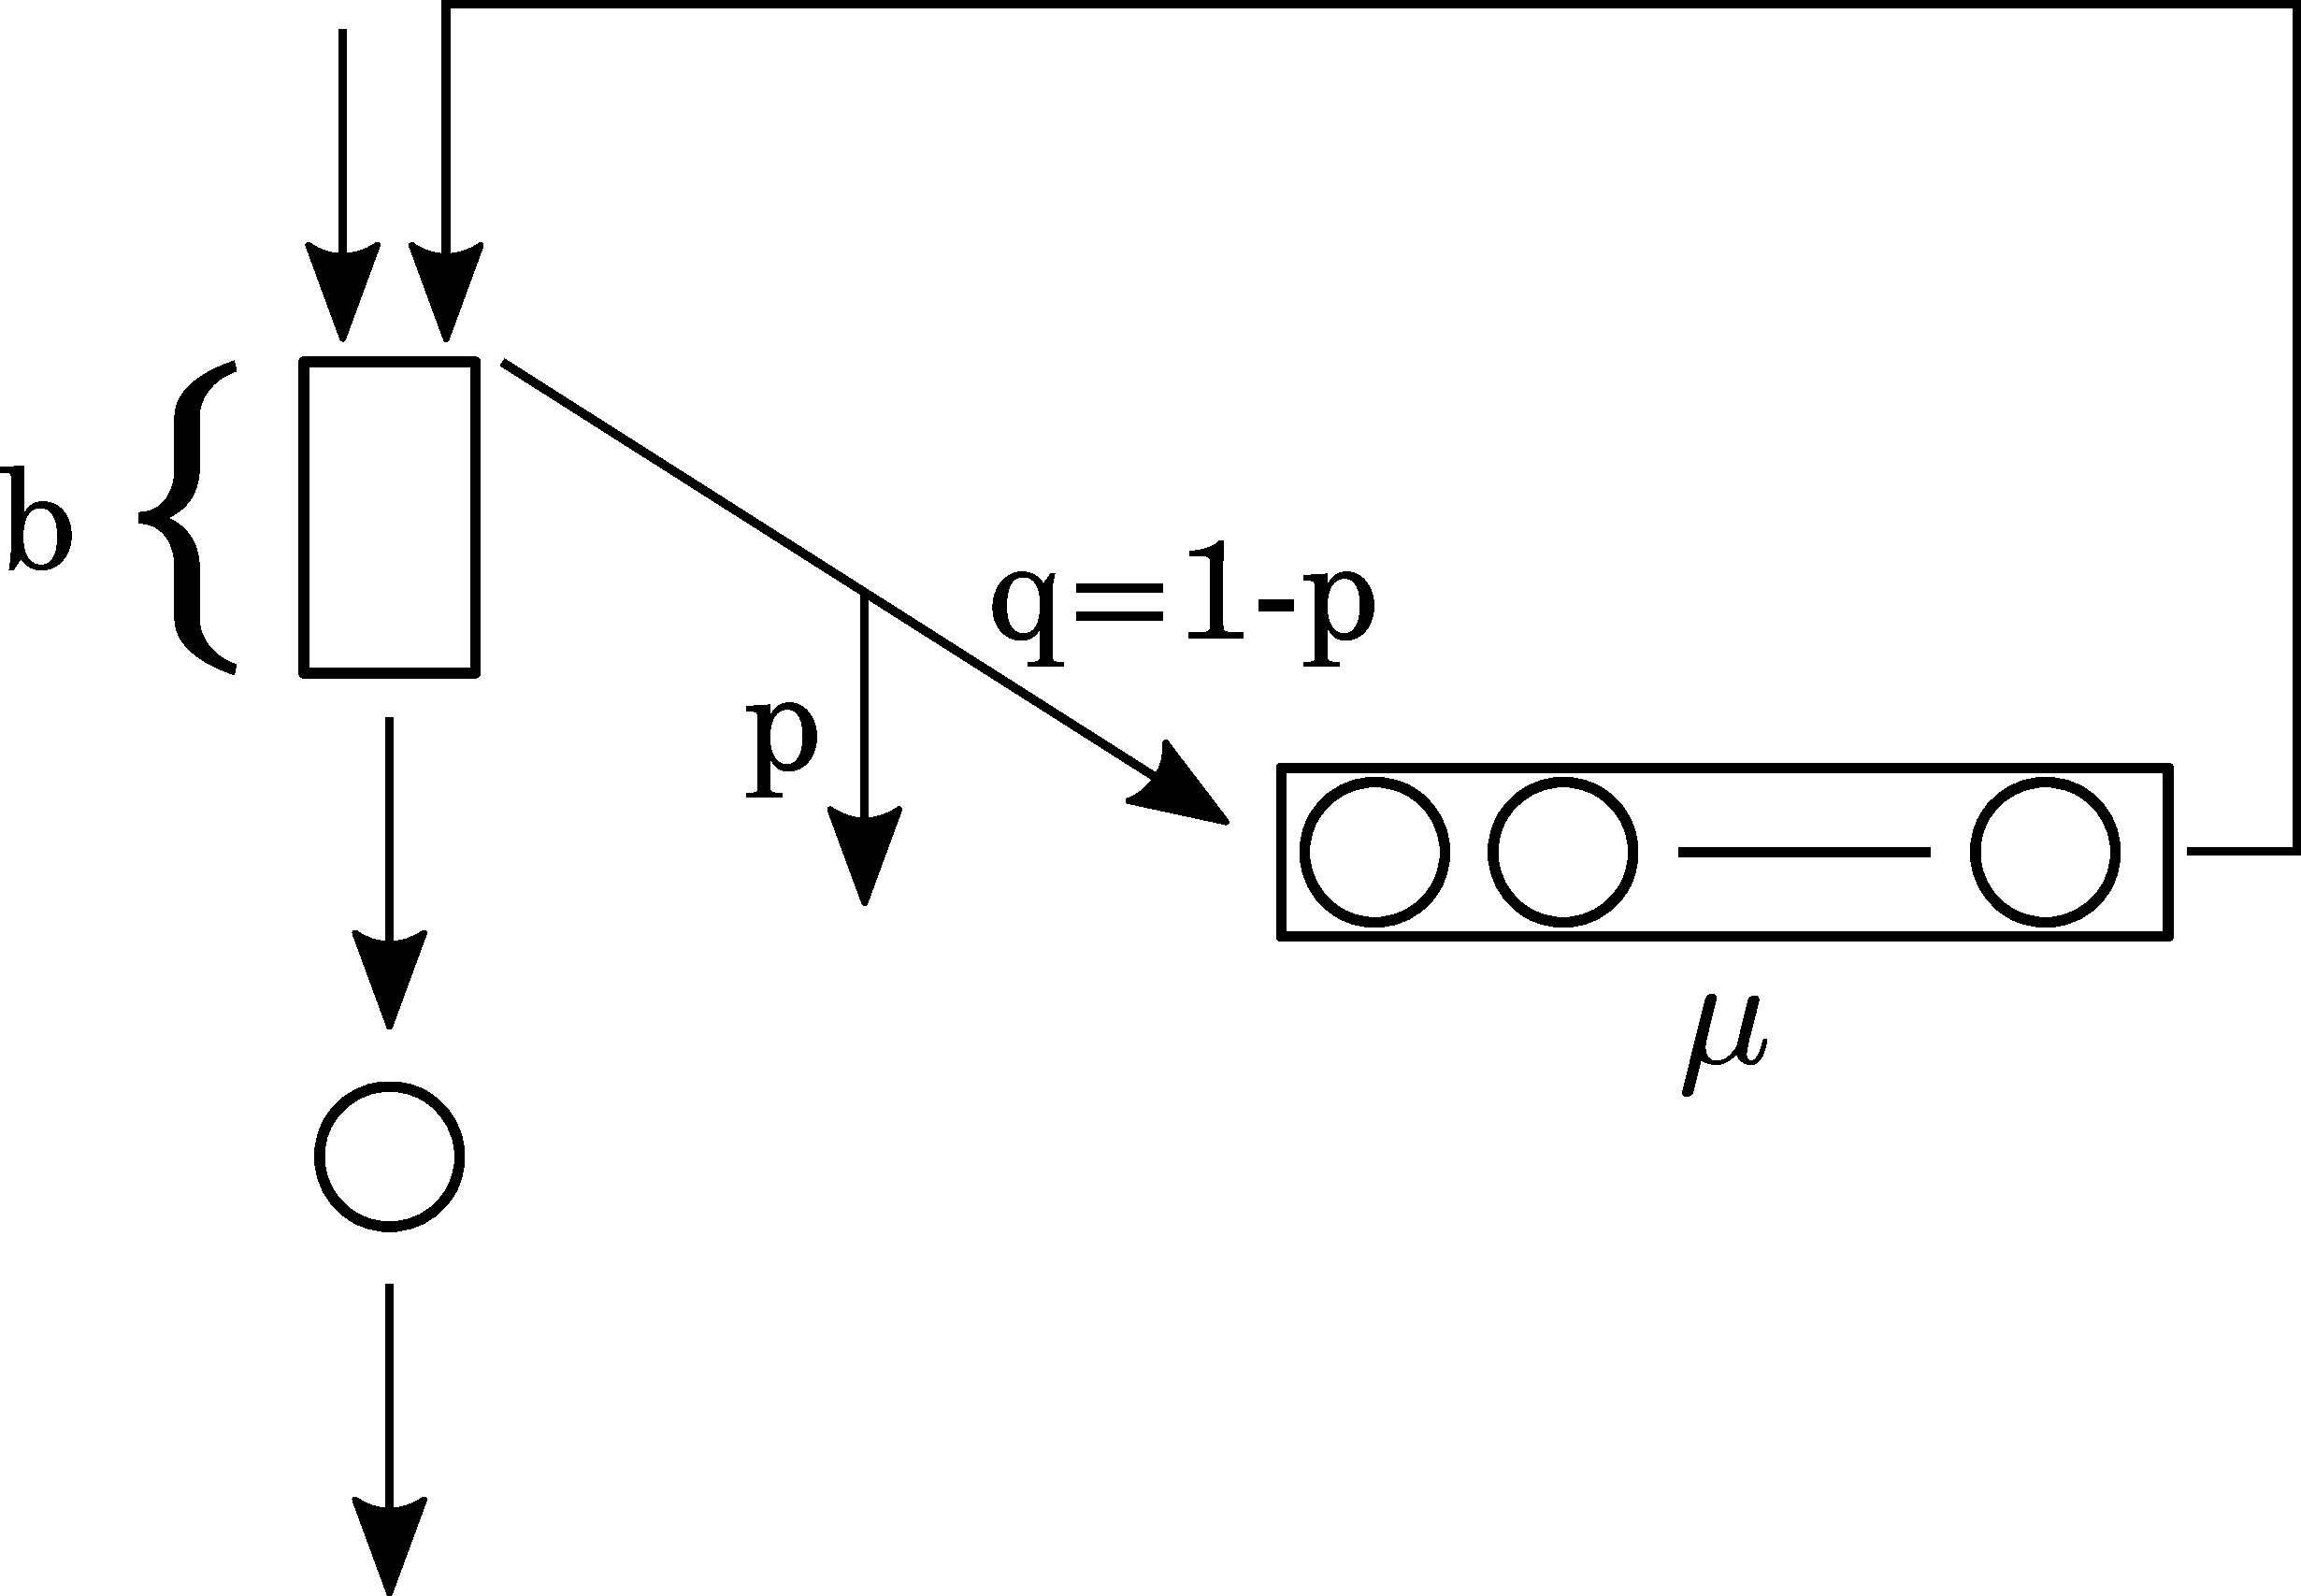
\includegraphics[width=0.7\textwidth]{pictures/p25.pdf}
  \end{center}
\end{frame}

%\subsection{Model and Assumptions}
%%%%%%%%%%%%%%%%%%%%%%%%%%%%%%%%%%%%
\begin{frame}
  \frametitle{The Model}
  % \framesubtitle{The Diffusion Scaled processes}
  \vfill

  \begin{tabular}{lc}
	\begin{tabular}{l}
	  \parbox{0.5\linewidth}{
		{\bf $2$ stations:} \textcolor[RGB]{00,136,00}{main} and \textcolor[RGB]{128,00,128} {retrial}.
		\begin{itemize}
		\item <2-> \textcolor[RGB]{00,136,00}{Main station:}
		  \begin{itemize}
          \item <2-> $G/G/1$ queue, finite buffer size b.
          \item <3-> Reject incoming customers when buffer full.
          \item <4-> Each rejected customer move to the retrial station w.p. q.
          \end{itemize}
        \item <5-> \textcolor[RGB]{128,00,128} {Retrial station:}
          \begin{itemize}
          \item <5-> Infinite number of exponential servers. 
          \item <6-> Service rate $\mu$. 
          \end{itemize}
		  
	  \end{itemize}}
	\end{tabular}	
	& \begin{tabular}{c}
	    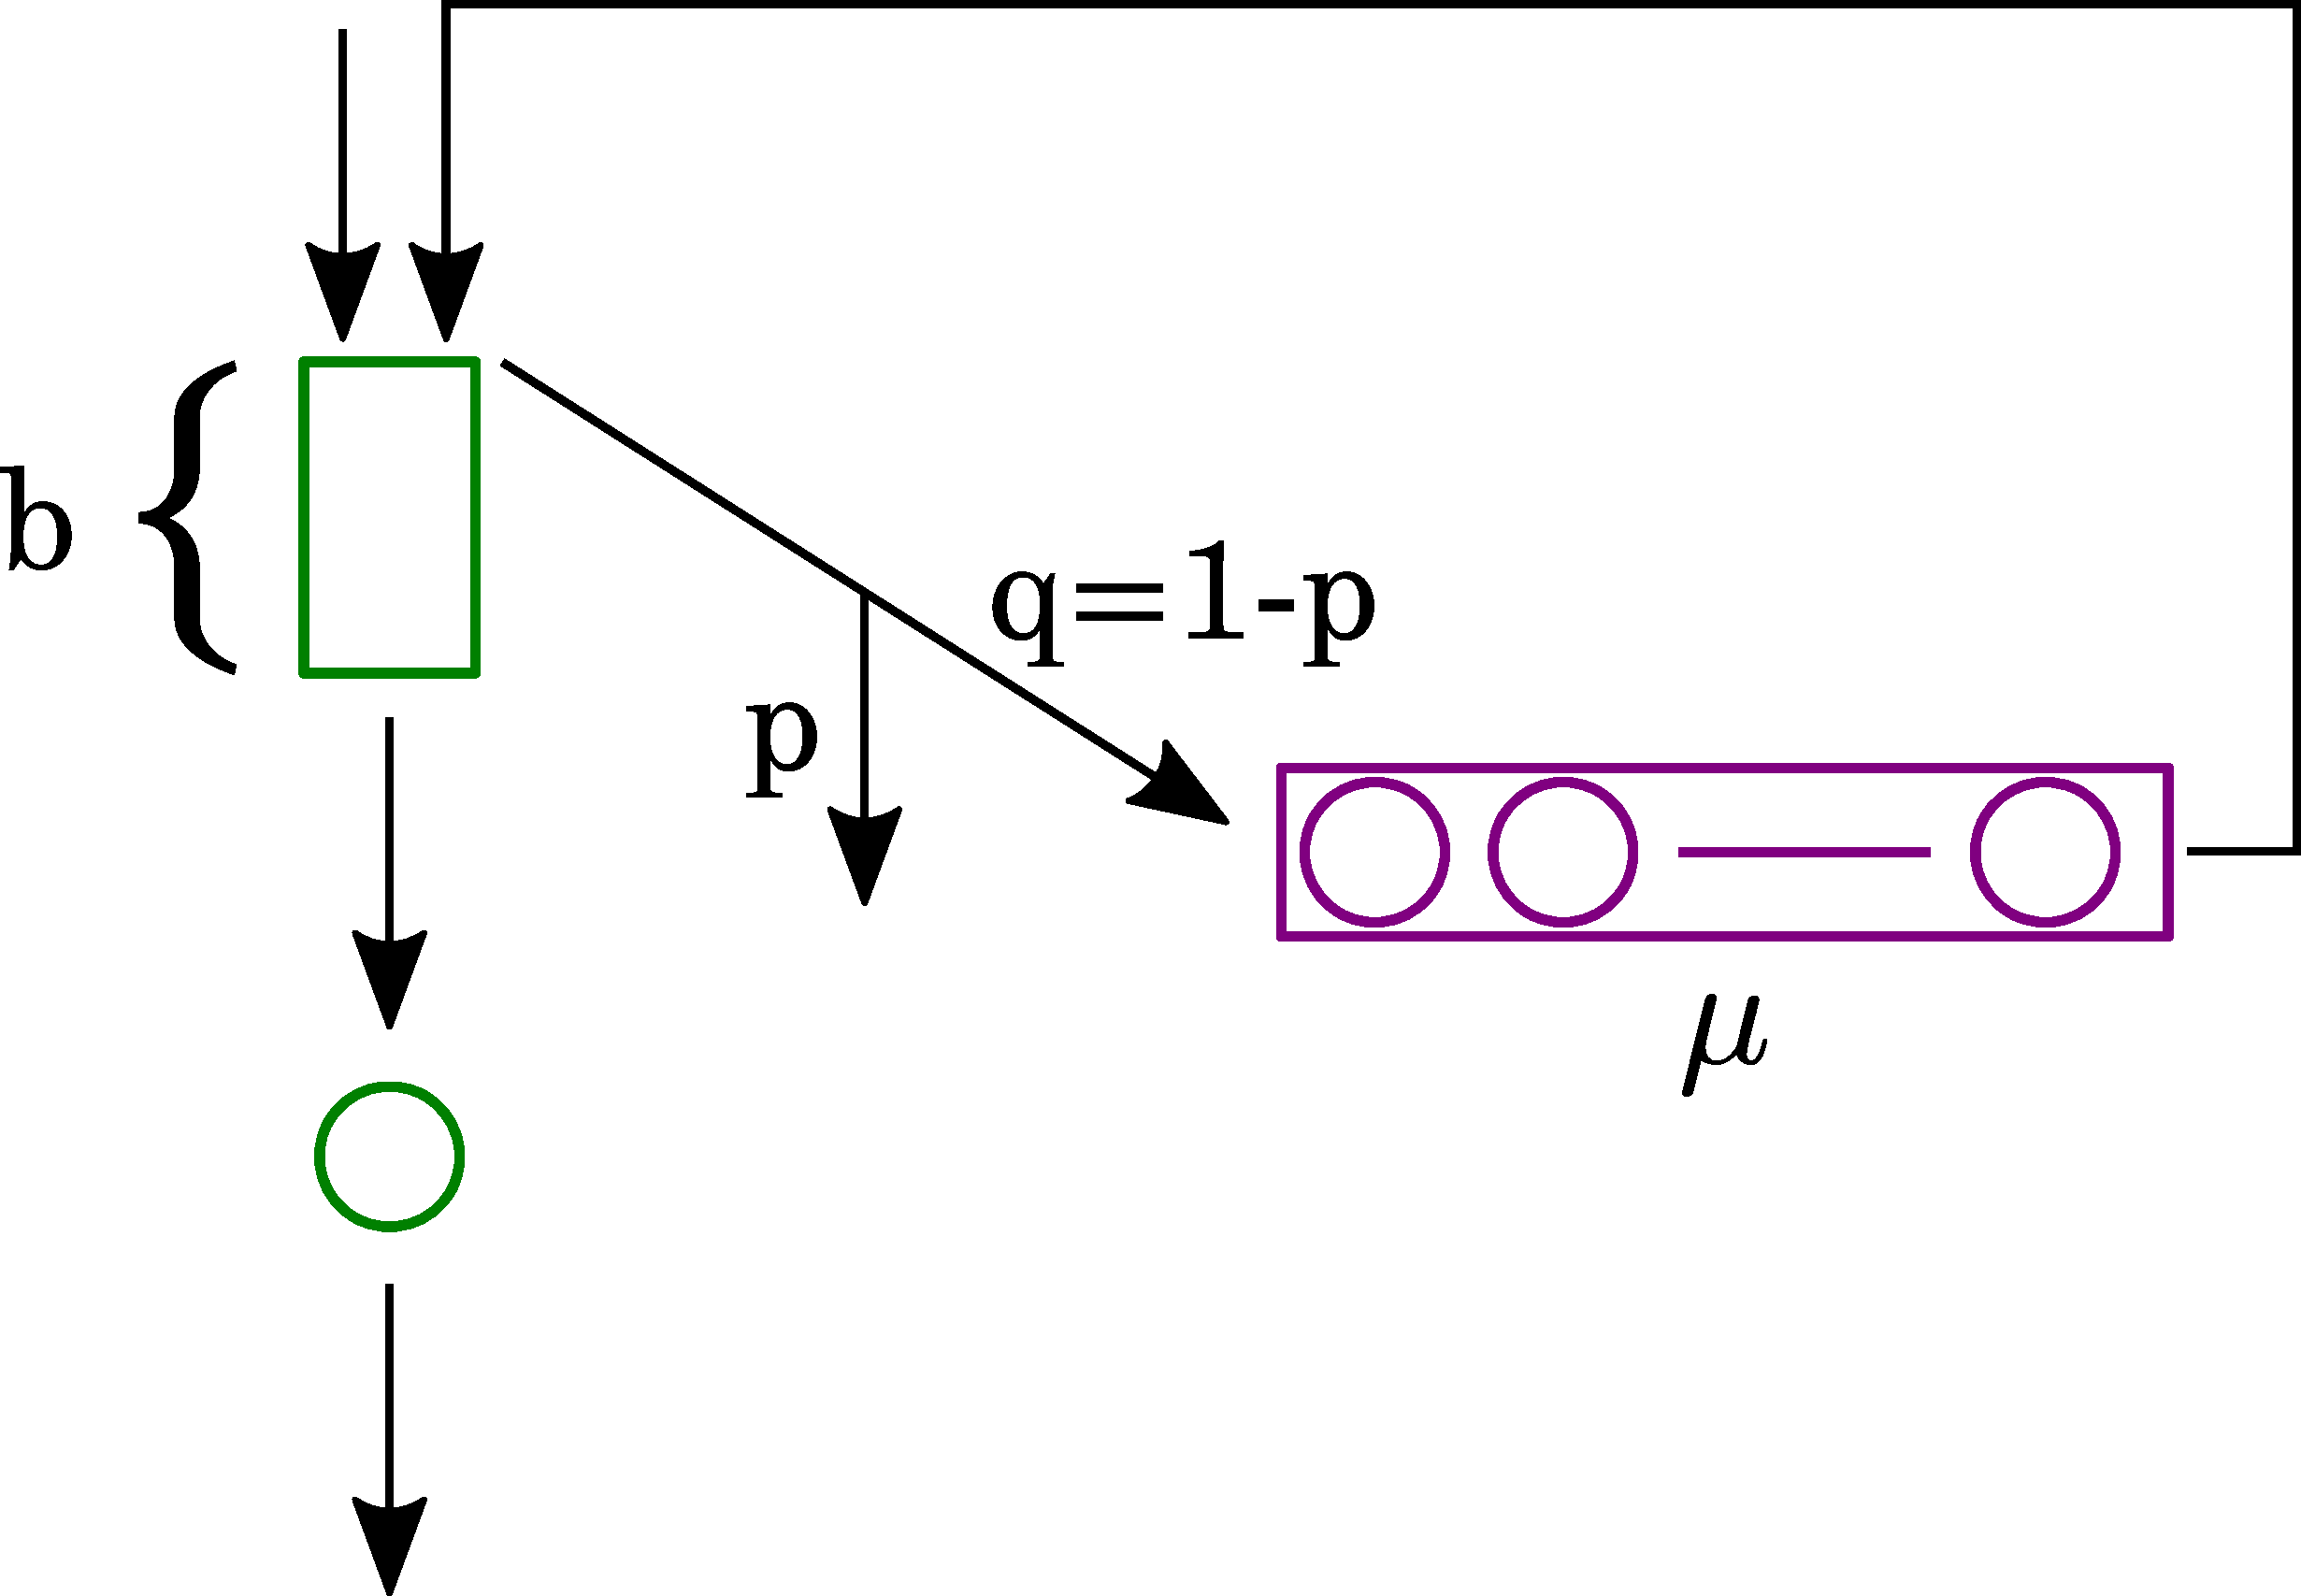
\includegraphics[width=0.4\linewidth]{pictures/p25_1.pdf}
	  \end{tabular} \\
  \end{tabular}

  \vfill
  \only<7->{
    \begin{itemize}[<+->]
    \item {\bf First Problem:} Diffusion limits.
      \vfill
    \item {\bf Second Problem:} Optimizing b with cost
      \[
      \mathbb{E} \int_{0}^{\infty} e^{-\alpha t} (c_1 \underbrace{X(t)}_\text{system state}dt+c_2 d\underbrace{C(t)}_\text{rejections count})
      \]  

    \end{itemize}

  }
  \vfill
\end{frame}



\begin{frame}
  \frametitle{Related Work}
  %\framesubtitle{The diffusion scale}

\begin{enumerate}
\item \bibentry{mandelbaum1998strong}
%\item \bibentry{anisimov1999switching}
\item \bibentry{falin1995approximations}
\end{enumerate}



\end{frame}

\begin{frame}
  \frametitle{First Problem - The Diffusion Limits}
  \framesubtitle{The Diffusion Model}

  \vfill
  \begin{itemize}[<+->]
  \item As before, use diffusion scale to arrive to the diffusion model.
    \vfill
  \item The diffusion model consists of:
    \begin{itemize}
    \item $X(t)$- number of customers in the main station (at time $t$).\\
    \item $R(t)$- number of customers in the retrial station (at time $t$).\\
    \item $C(t)$ - rejections count, $L(t)$ - idle time. Keep the process $X$ in $[0,b]$.
    \end{itemize}
    \vfill

  \item The diffusion model is characterize using the Skorokhod Map on $[0,b]$. 
  \end{itemize}
  \vfill

\end{frame}

\begin{frame}
\frametitle{First Problem - The Diffusion Limits}  
  \framesubtitle{The Skorokhod Map on $[0,b]$}
%\framesubtitle{(Kruk Lehoczky Ramanan Shreve $07'$) }

  \vfill
  \onslide<+->{
    \begin{definition}{\bf The Skorokhod Problem on $[0,b]$ (Tanaka $'79$)}


      Given $\psi\in\calD[0,\iy)$, find $(\phi, \eta_l, \eta_u )\in(\calD[0,\iy))^3$, such that
          \begin{enumerate}
          \item $\phi(t)=\psi(t) + \eta_l(t)-\eta_u(t), \qquad \phi(t)\in [0,b] \qquad \text{for all $t$}$.
          \item $\eta_l,\eta_u$ are non negative and non decreasing and one has
            \[
            \int_{[0,\infty)} \mathbb{I}_{\{\phi(t)>0\}} d\eta_l(t)=0, \qquad
              \int_{[0,\infty)} \mathbb{I}_{\{\phi(t)<b\}} d\eta_u(t)=0.
                \]
          \end{enumerate}

          
    \end{definition}
              }
              \vfill
              \begin{itemize}[<+->]
                %\item $\phi$ behaves as $\psi$ in $(0,b)$. $\eta_l(t),\eta_u(t)$ push $\phi$ inside $[0,b]$ when it reaches the boundaries.  
                %\vfill
              \item Has a unique solution.
                \vfill
              \item The solution is called the {\it Skorohod map} and is denoted by $\Gamma_{0,b}$.
                \vfill
              \item Thus $(\phi, \eta_l, \eta_u )=\Gamma_{0,b}(\psi)$.
              \end{itemize}
              \vfill

\end{frame}


%%%%%%%%%%%%%%%%%%%%%%%%%%%%%%%
\begin{frame}
  \frametitle{First Problem - The Diffusion Limits}  
  \framesubtitle{The Diffusion Model Definition}
  % \framesubtitle{The diffusion scale}

  \vfill
  \onslide<+->{
    \begin{equation*}\label{Diffmodel}
      \begin{dcases}
        (X, L, C)=\Gamma_{0,b}(Z)\\
        Z(t)=x+\underbrace{W(t)}_\text{BM}+\int_0^t \mu R(s)ds \\
        R(t)=r+qC(t)-\int_0^t \mu R(s)ds.\\
      \end{dcases}
    \end{equation*}
  }
  \vfill
  \onslide<+->{
    Reflection vector field: 
    \begin{center}
      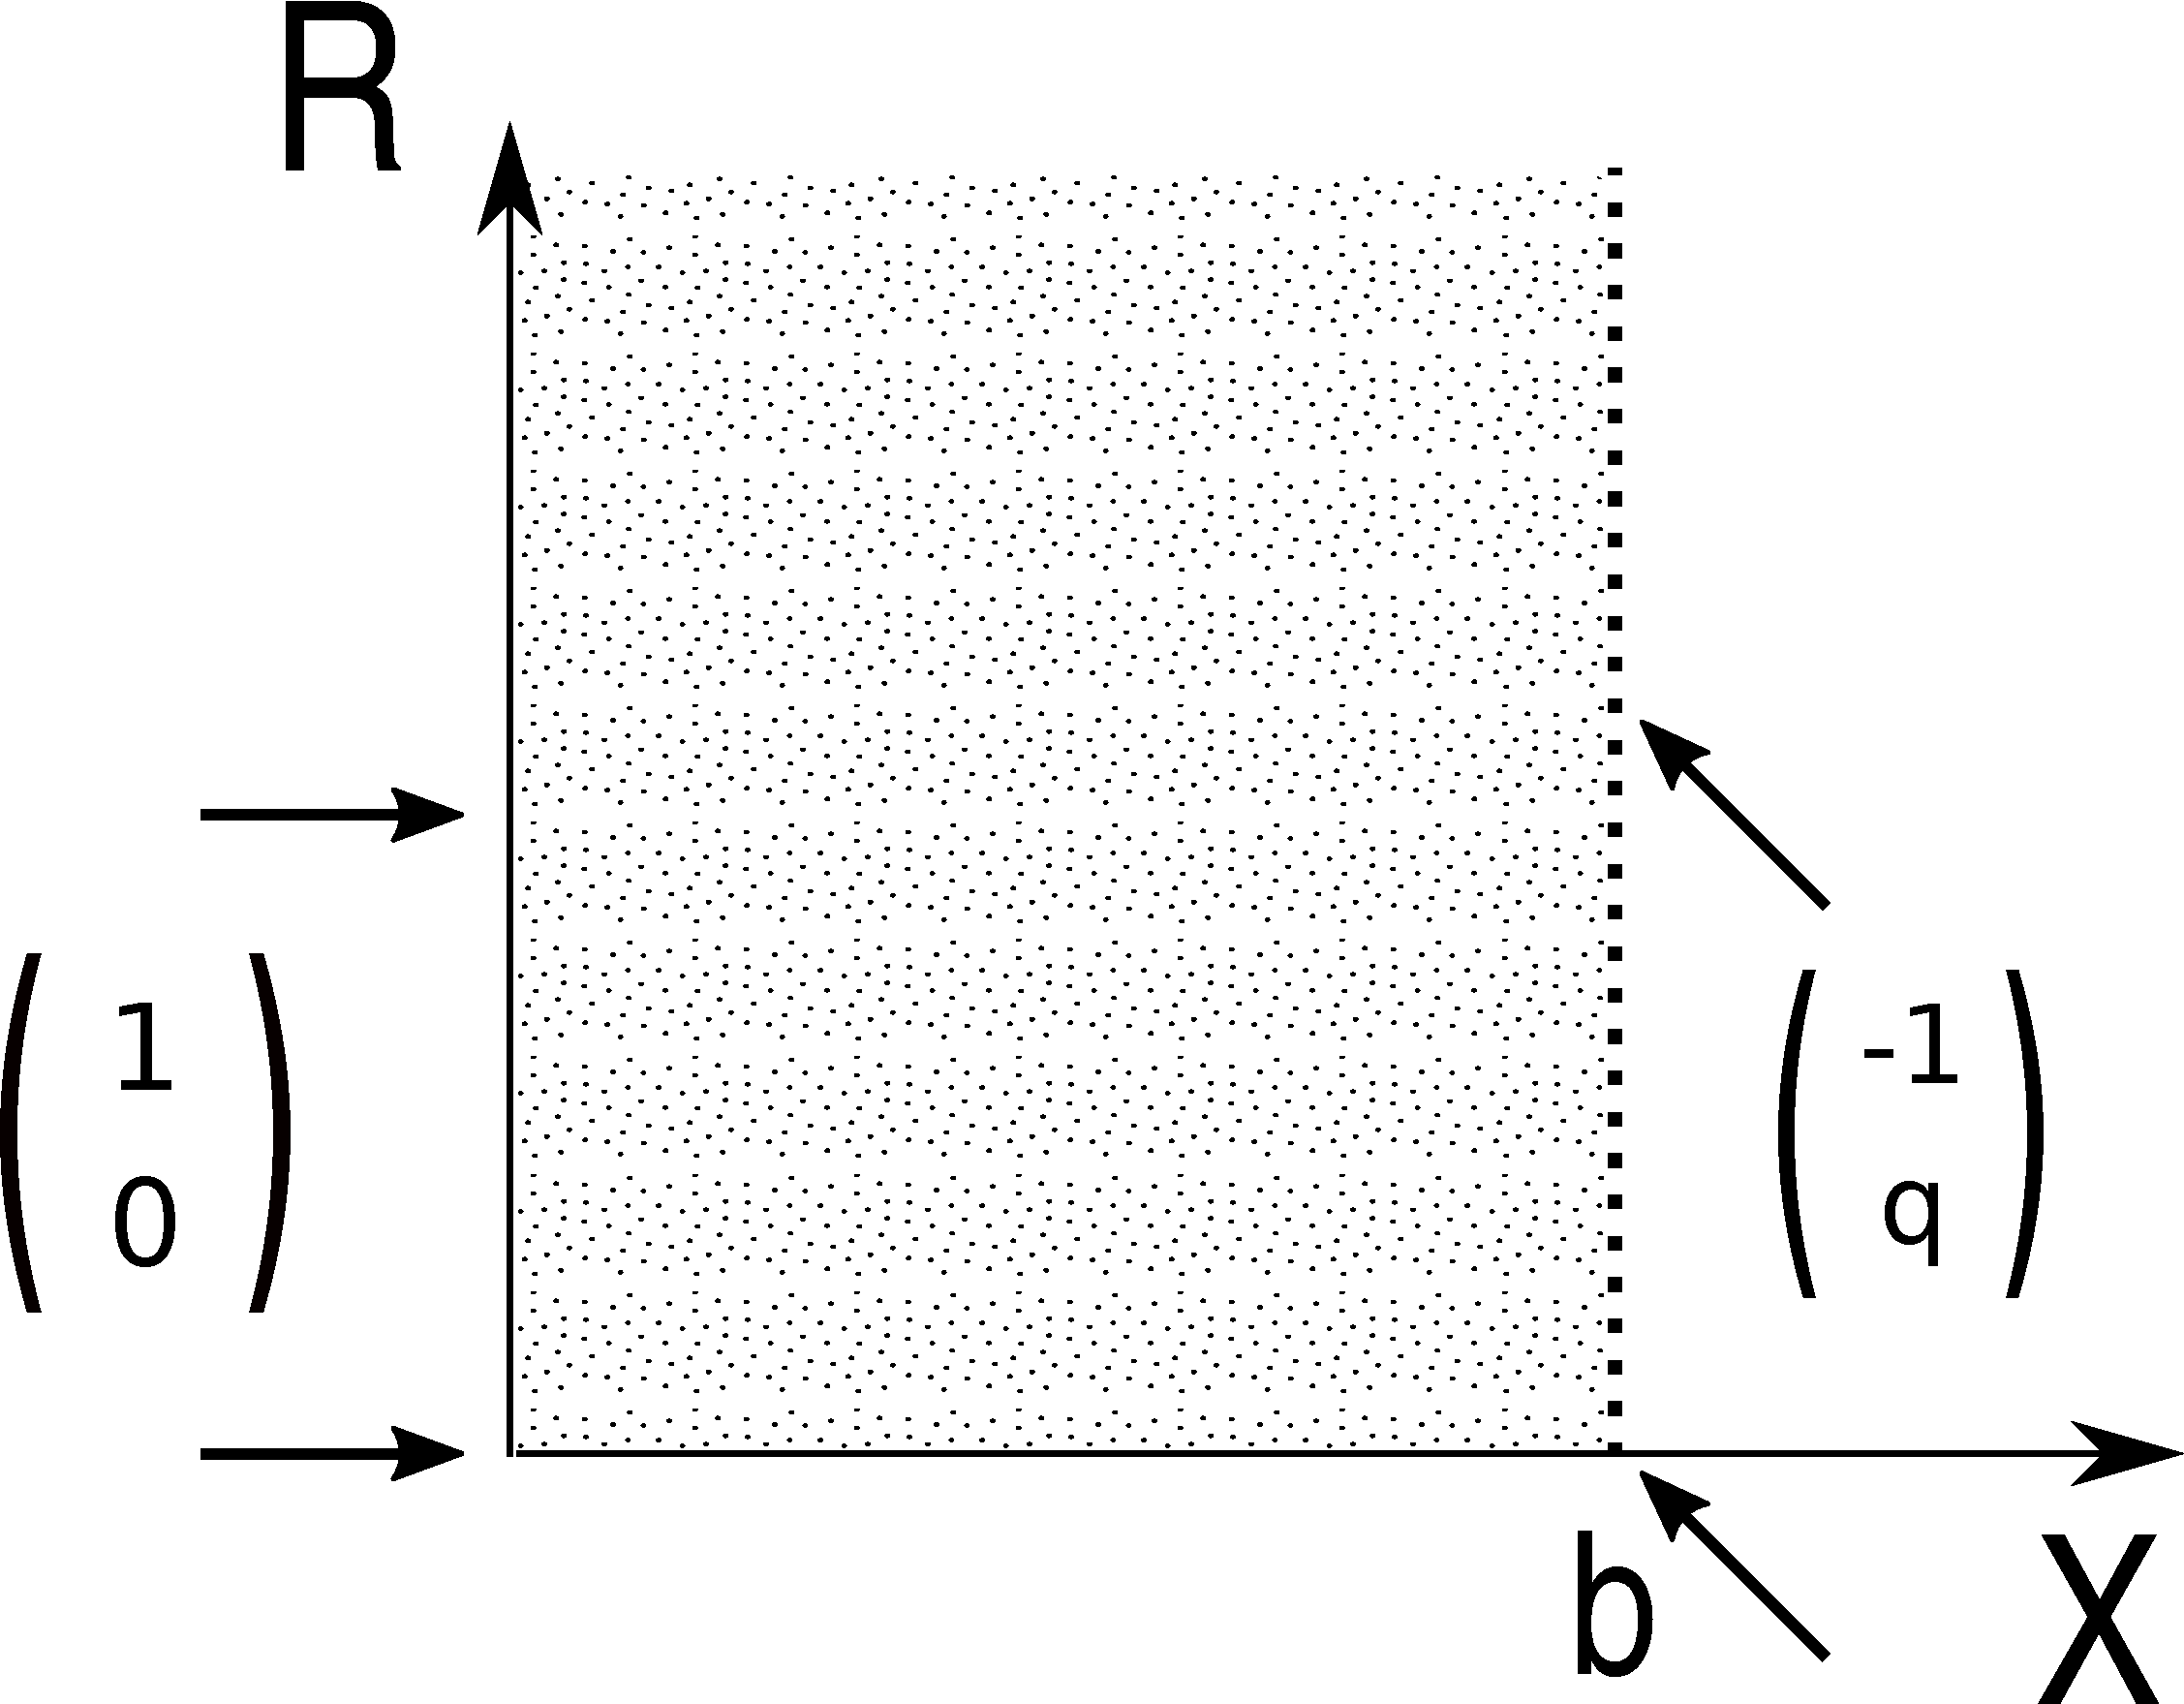
\includegraphics[width=0.3\textwidth]{pictures/diffReflection.pdf}
    \end{center}
  }
  \vfill
  \onslide<+->{
    {\bf Two dimensional reflected diffusion process which is degenerate in the second diffusion coefficient}
  }
\end{frame}

\subsection{First Result - Diffusion Limits}
\begin{frame}
  \frametitle{First Problem - The Diffusion Limits}  
  %\framesubtitle{The Diffusion Limits}

  \begin{theorem}\label{main}
    As $n\to \infty$,
    \[
    (\hat{X}^n, \hat{R}^n,\hat L^n,\hat C^n)\Rightarrow (X,R,L,C).
    \]
  \end{theorem}

  
\end{frame}



%%%%%%%%%%%%%%%%%%%%%%%%%%%%%%%%%%%%%%%%%%%%%%%%%%%%%%%%%%
\subsection{Second Result - Optimal Buffer Size}
%%%%%%%%%%%%%%%%%%%%%%%%%%%%%%%%%%%%%%%%%%%%%%%%%%%%%%%%%%%%%
\begin{frame}
  \frametitle{Second Result - The Diffusion Optimization Problem}
  \framesubtitle{Definition}

  \vfill
  \begin{itemize}[<+->]
  \item {\bf Cost:}  
    \[
    \mathbb{E} \Big(\int_{0}^{\infty} e^{-\alpha t} (c_1 X(t)dt+c_2 dC(t))\Big)
    \]
    \vfill
  \item {\bf Not solvable as before:}
    \begin{enumerate}[<+->]%
    \item Not solvable explicitly - the Bellman equation is in two dimensions (correspond to $(X,R)$)
    \item Not applicable - the solution require knowledge of the number of customers in retrial (not observable).  
    \end{enumerate}
    \vfill
  \item {\bf New Goal:} Optimize over buffer size b (using the diffusion model). 
\vfill
\item {\bf Value:}
   \[
    V(x)=\inf_{b} \mathbb{E} \Big(\int_{0}^{\infty} e^{-\alpha t} (c_1 X(t)dt+c_2 dC(t))\Big)
    \]
  \end{itemize}
  \vfill 
\end{frame}

\begin{frame}
  \frametitle{Second Result - The Diffusion Optimization Problem}
  \framesubtitle{Solution}

  \vfill
  \begin{itemize}[<+->]%
  \item Reduction to a $1$-dimensional problem (SSC) for: 

    \begin{enumerate}[<+->]%
    \item $\mu \to 0$
    \item $\mu \to \infty$
    \end{enumerate}
    \vfill
  \item For general $\mu\in (0,\infty)$ - simulation.

  \end{itemize}
  \vfill

\end{frame}


\begin{frame}
\frametitle{Second Result - The Diffusion Optimization Problem}
  \framesubtitle{The Harrison-Taksar Free Boundary Problem}
   %\framesubtitle{(Harrison Taksar $83'$)}

  \vfill
  \begin{itemize}[<+->]%
  \item Harrison Taksar $'83$.
  \vfill  
  \item $1$-dimensional problem.
    \vfill
  \item One server, infinite queue. No retrials.
    \vfill
  \item Controls the buffer size to minimize the same cost.
  \end{itemize}
  \vfill

\end{frame}


\begin{frame}
  \frametitle{Second Result - The Diffusion Optimization Problem}
  \framesubtitle{The Harrison-Taksar Free Boundary Problem}

  \vfill
  \onslide<+->{
    \begin{equation*}
      \begin{multlined}
        \begin{cases}
          (\tilde X, \tilde L, \tilde C)=\Gamma_{0,b}(x+W), \qquad \text{where $W$ is a BM}\\    
          J_\HT^b[x;c_1,c_2]=\mathbb{E}\int_0^\iy e^{-\al t}[c_1\tilde X_t+c_2\tilde C_t]dt,
        \end{cases}    
      \end{multlined}
    \end{equation*}
  }
  \vfill
  \begin{itemize}[<+->]
  \item Has a unique optimal buffer size: $b_\HT[c_1,c_2]$ .
    \vfill
  \item The value function
    
    \begin{equation*}\label{040}
      v[x;c_1,c_2]=\inf_{b\in(0,\iy)}J_{\HT}^b[x;c_1,c_2].
    \end{equation*}
    is the unique solution to a $1$-dimensional Bellman equation:
    \begin{equation*}
   \begin{cases}
    \ds\frac{1}{2}\sig^2f''+\hat yf'-\al f+c_1=0,
    &\text{ in } (0,b_0),\\ \\
    \ds f'(0)=0,\qquad f'(b_0)=\frac{c_2}{\al}.
  \end{cases}
\end{equation*}
(unknowns: $f$ and $b_0$)
  \end{itemize}
  \vfill
\end{frame}


\begin{frame}
\frametitle{Second Result - The Diffusion Optimization Problem}
   \framesubtitle{The Case $\mu\to 0$}
  %  \framesubtitle{The diffusion scale}

  \begin{theorem}
    \label{th2}
    One has
    \[
    \liminf_{\mu\to0}\liminf_{n\to\iy}V^{n,\mu}
    =\limsup_{\mu\to0}\limsup_{n\to\iy}V^{n,\mu}=v[x;c_1,c_2],
    \]
    and $b_\HT[c_1,c_2]$ is an AO scaled buffer size, namely, with
    $b=b_\HT[c_1,c_2]$,
    \[
    \liminf_{\mu\to 0}\liminf_{n\to\iy}J^{n,\mu,b}
    =\limsup_{\mu\to 0}\limsup_{n\to\iy}J^{n,\mu,b}=v[x;c_1,c_2].
    \]
  \end{theorem}


\end{frame}

\begin{frame}
\frametitle{Second Result - The Diffusion Optimization Problem}
   \framesubtitle{The Case $\mu \to \infty$}
  %\framesubtitle{The diffusion scale}

  \begin{theorem}
    \label{th1}
    One has
    \[
    \liminf_{\mu\to\iy}\liminf_{n\to\iy}V^{n,\mu}
    =\limsup_{\mu\to\iy}\limsup_{n\to\iy}V^{n,\mu}=v[x;c_1,\frac{c_2}{p}].
    \]
    Moreover, $b_\HT[c_1,\frac{c_2}{p}]$ is an AO scaled buffer size,
    in the sense that, with $b=b_\HT[c_1,\frac{c_2}{p}]$,
    \[
    \liminf_{\mu\to\iy}\liminf_{n\to\iy}J^{n,\mu,b}
    =\limsup_{\mu\to\iy}\limsup_{n\to\iy}J^{n,\mu,b}=v[x;c_1,\frac{c_2}{p}].
    \]
  \end{theorem}

\end{frame}

\subsection{Simulation}


\begin{frame}
  \frametitle{Simulation}
  \framesubtitle{Buffer Size, $\mu \in [0,5000]$}
  \begin{center}
    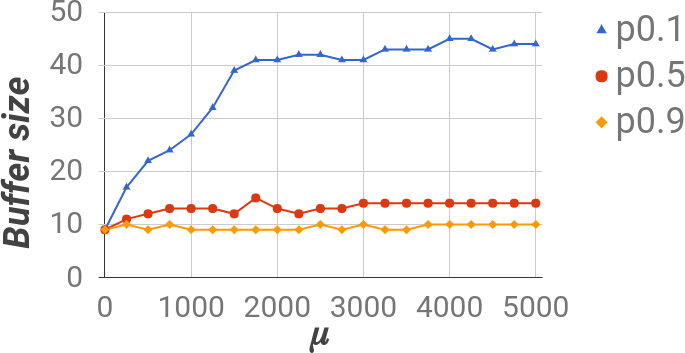
\includegraphics[width=1\textwidth]{pictures/bsim0-5000.png}
  \end{center}

\end{frame}

\begin{frame}
  \frametitle{Simulation}
  \framesubtitle{Value Function, $\mu \in [0,5000]$}

  \begin{center}
    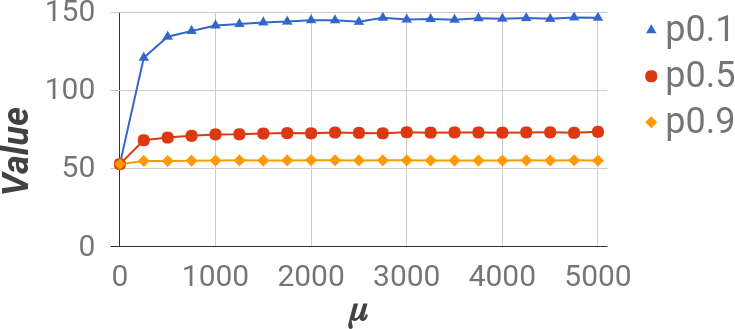
\includegraphics[width=1.0\textwidth]{pictures/vsim0-5000.png}
  \end{center}

\end{frame}

\begin{frame}
  \frametitle{Simulation}
  \framesubtitle{Buffer Size, $\mu \in [0,0.01]$}  
  \begin{center}
    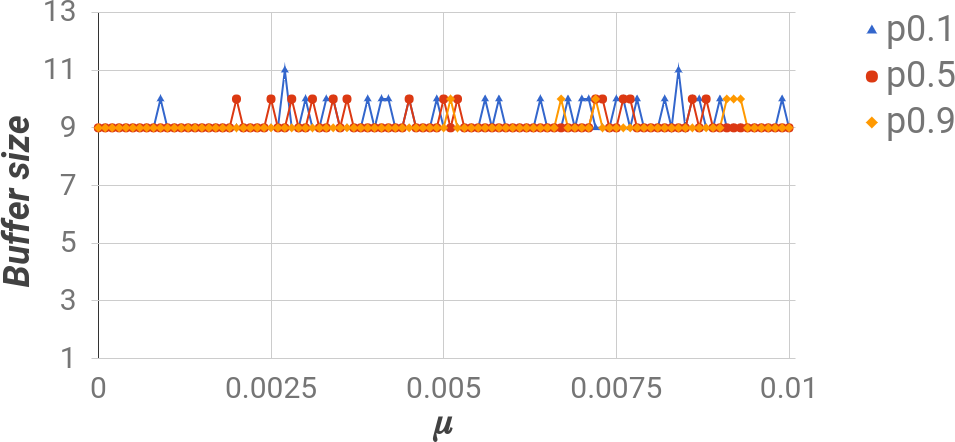
\includegraphics[width=1.0\textwidth]{pictures/bsim0-001.png}
  \end{center}

\end{frame}

\begin{frame}
 \frametitle{Simulation}
  \framesubtitle{Value of $\mu \in [0,0.01]$}
  \begin{center}
    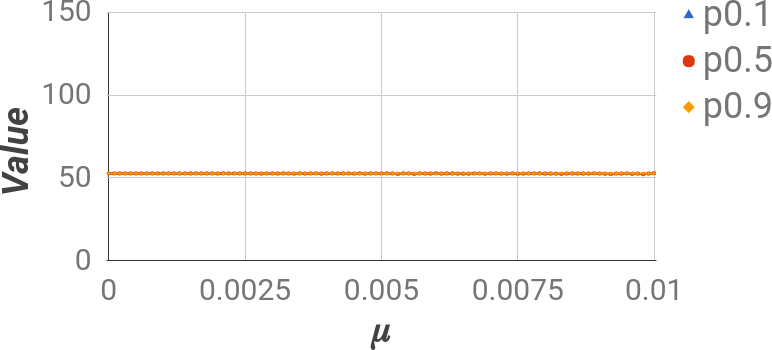
\includegraphics[width=1.0\textwidth]{pictures/vsim0-001.png}
  \end{center}

\end{frame}


\begin{frame}
 \frametitle{Simulation}
 \framesubtitle{Buffer Size, $\mu \in [4999,5000]$}  
 \begin{center}
    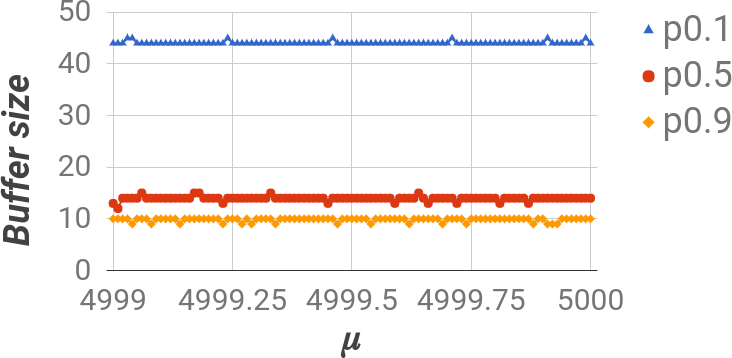
\includegraphics[width=1.0\textwidth]{pictures/bsim4999-5000.png}
  \end{center}
\end{frame}

\begin{frame}
  \frametitle{Simulation}
  \framesubtitle{Value Function, $\mu \in [4999,5000]$}
  \begin{center}
    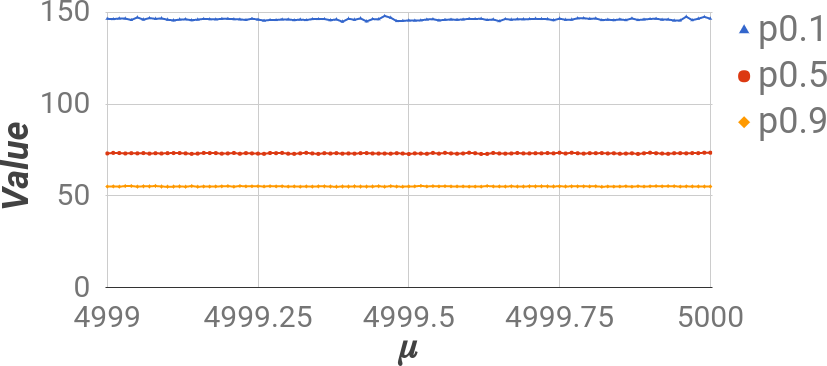
\includegraphics[width=1.0\textwidth]{pictures/vsim4999-5000.png}
  \end{center}
\end{frame}




%%%%%%%%%%%%%%%%%%%%%%%%%%%%%%%%%%%%%%%%%%%
\section{Acknowledgments}

\begin{frame}
  \frametitle{Acknowledgments}
  
\vfill
\begin{itemize}
\item {\bf Advisor:} Prof. Rami Atar
\vfill
%\item {\bf Team members:} Gal Mendelson, David Lipshutz,  Subhamay Saha, Anup Biswas
%\vfill
\item Probability group members
\vfill
\item {\bf Administration:} Orly Babad-Tamir and Danit Cohen
\vfill
%\item {\bf Scholarships:} 
%\begin{itemize}
%\item Israel and Debora Cederbaum Fellowship
%\item Freud award
%\end{itemize}
%\vfill
\item Andrew and Erna Viterbi Faculty of Electrical Engineering 
\end{itemize}  
\vfill
  
\end{frame}  


\begin{frame}
  \frametitle{Acknowledgments}

\vfill  
    \begin{center}
      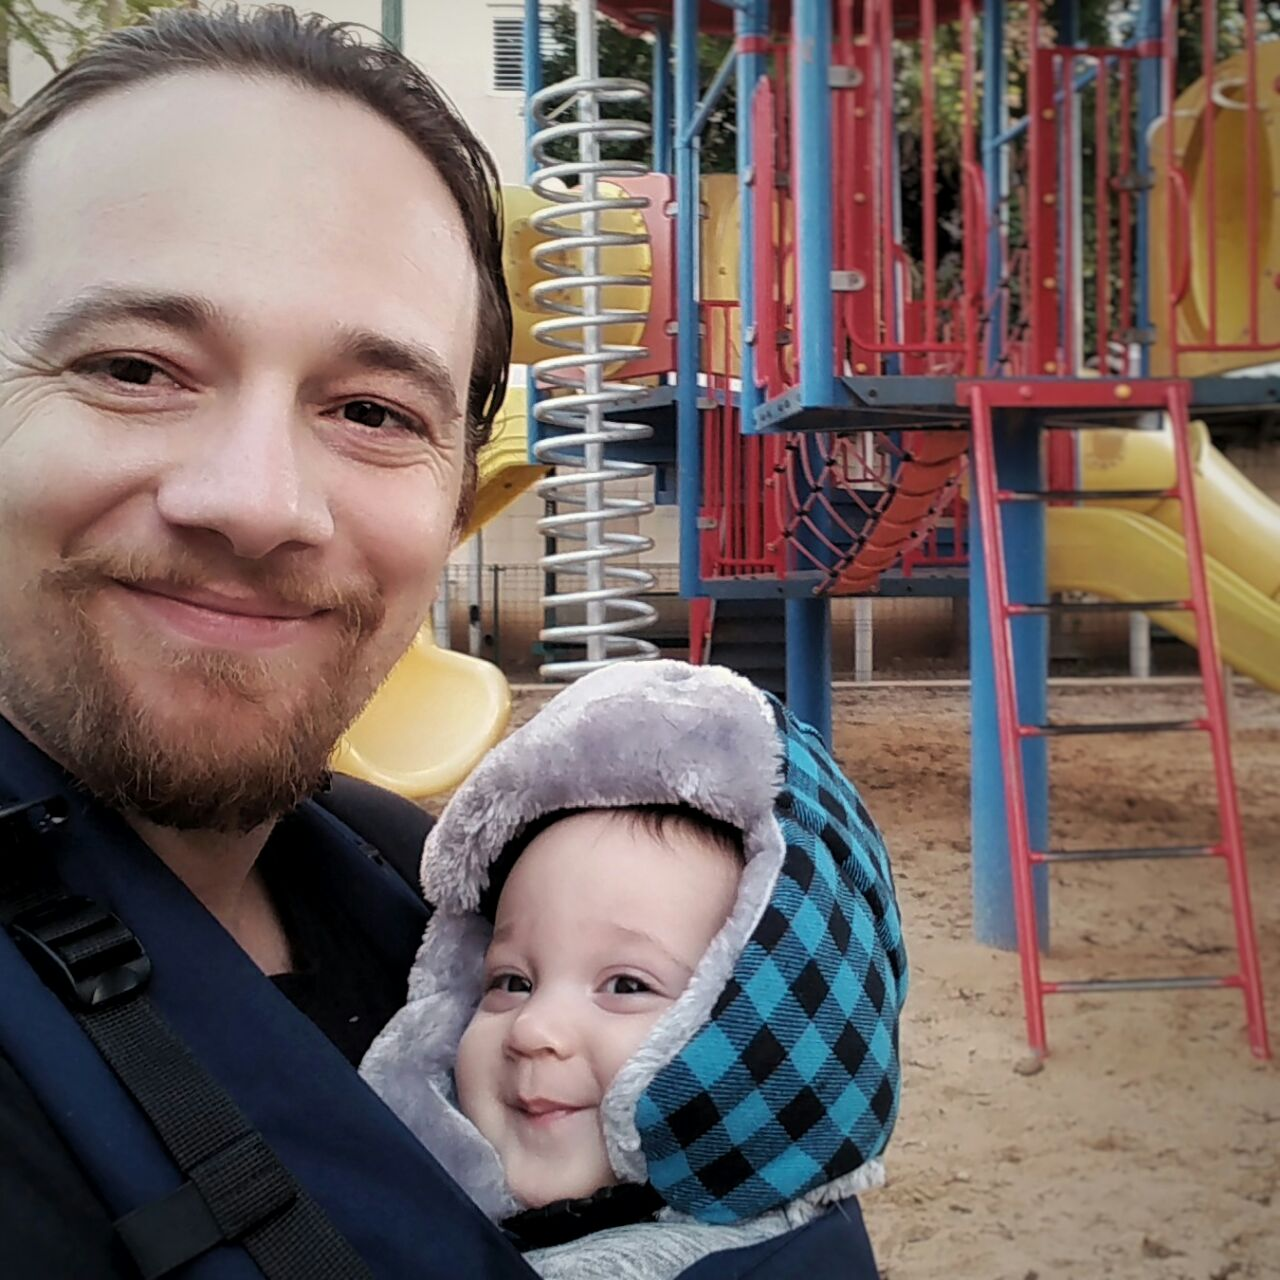
\includegraphics[width=0.3\textwidth]{pictures/KfirandAdam.jpg}
    \end{center}
\vfill    
    \begin{center}
      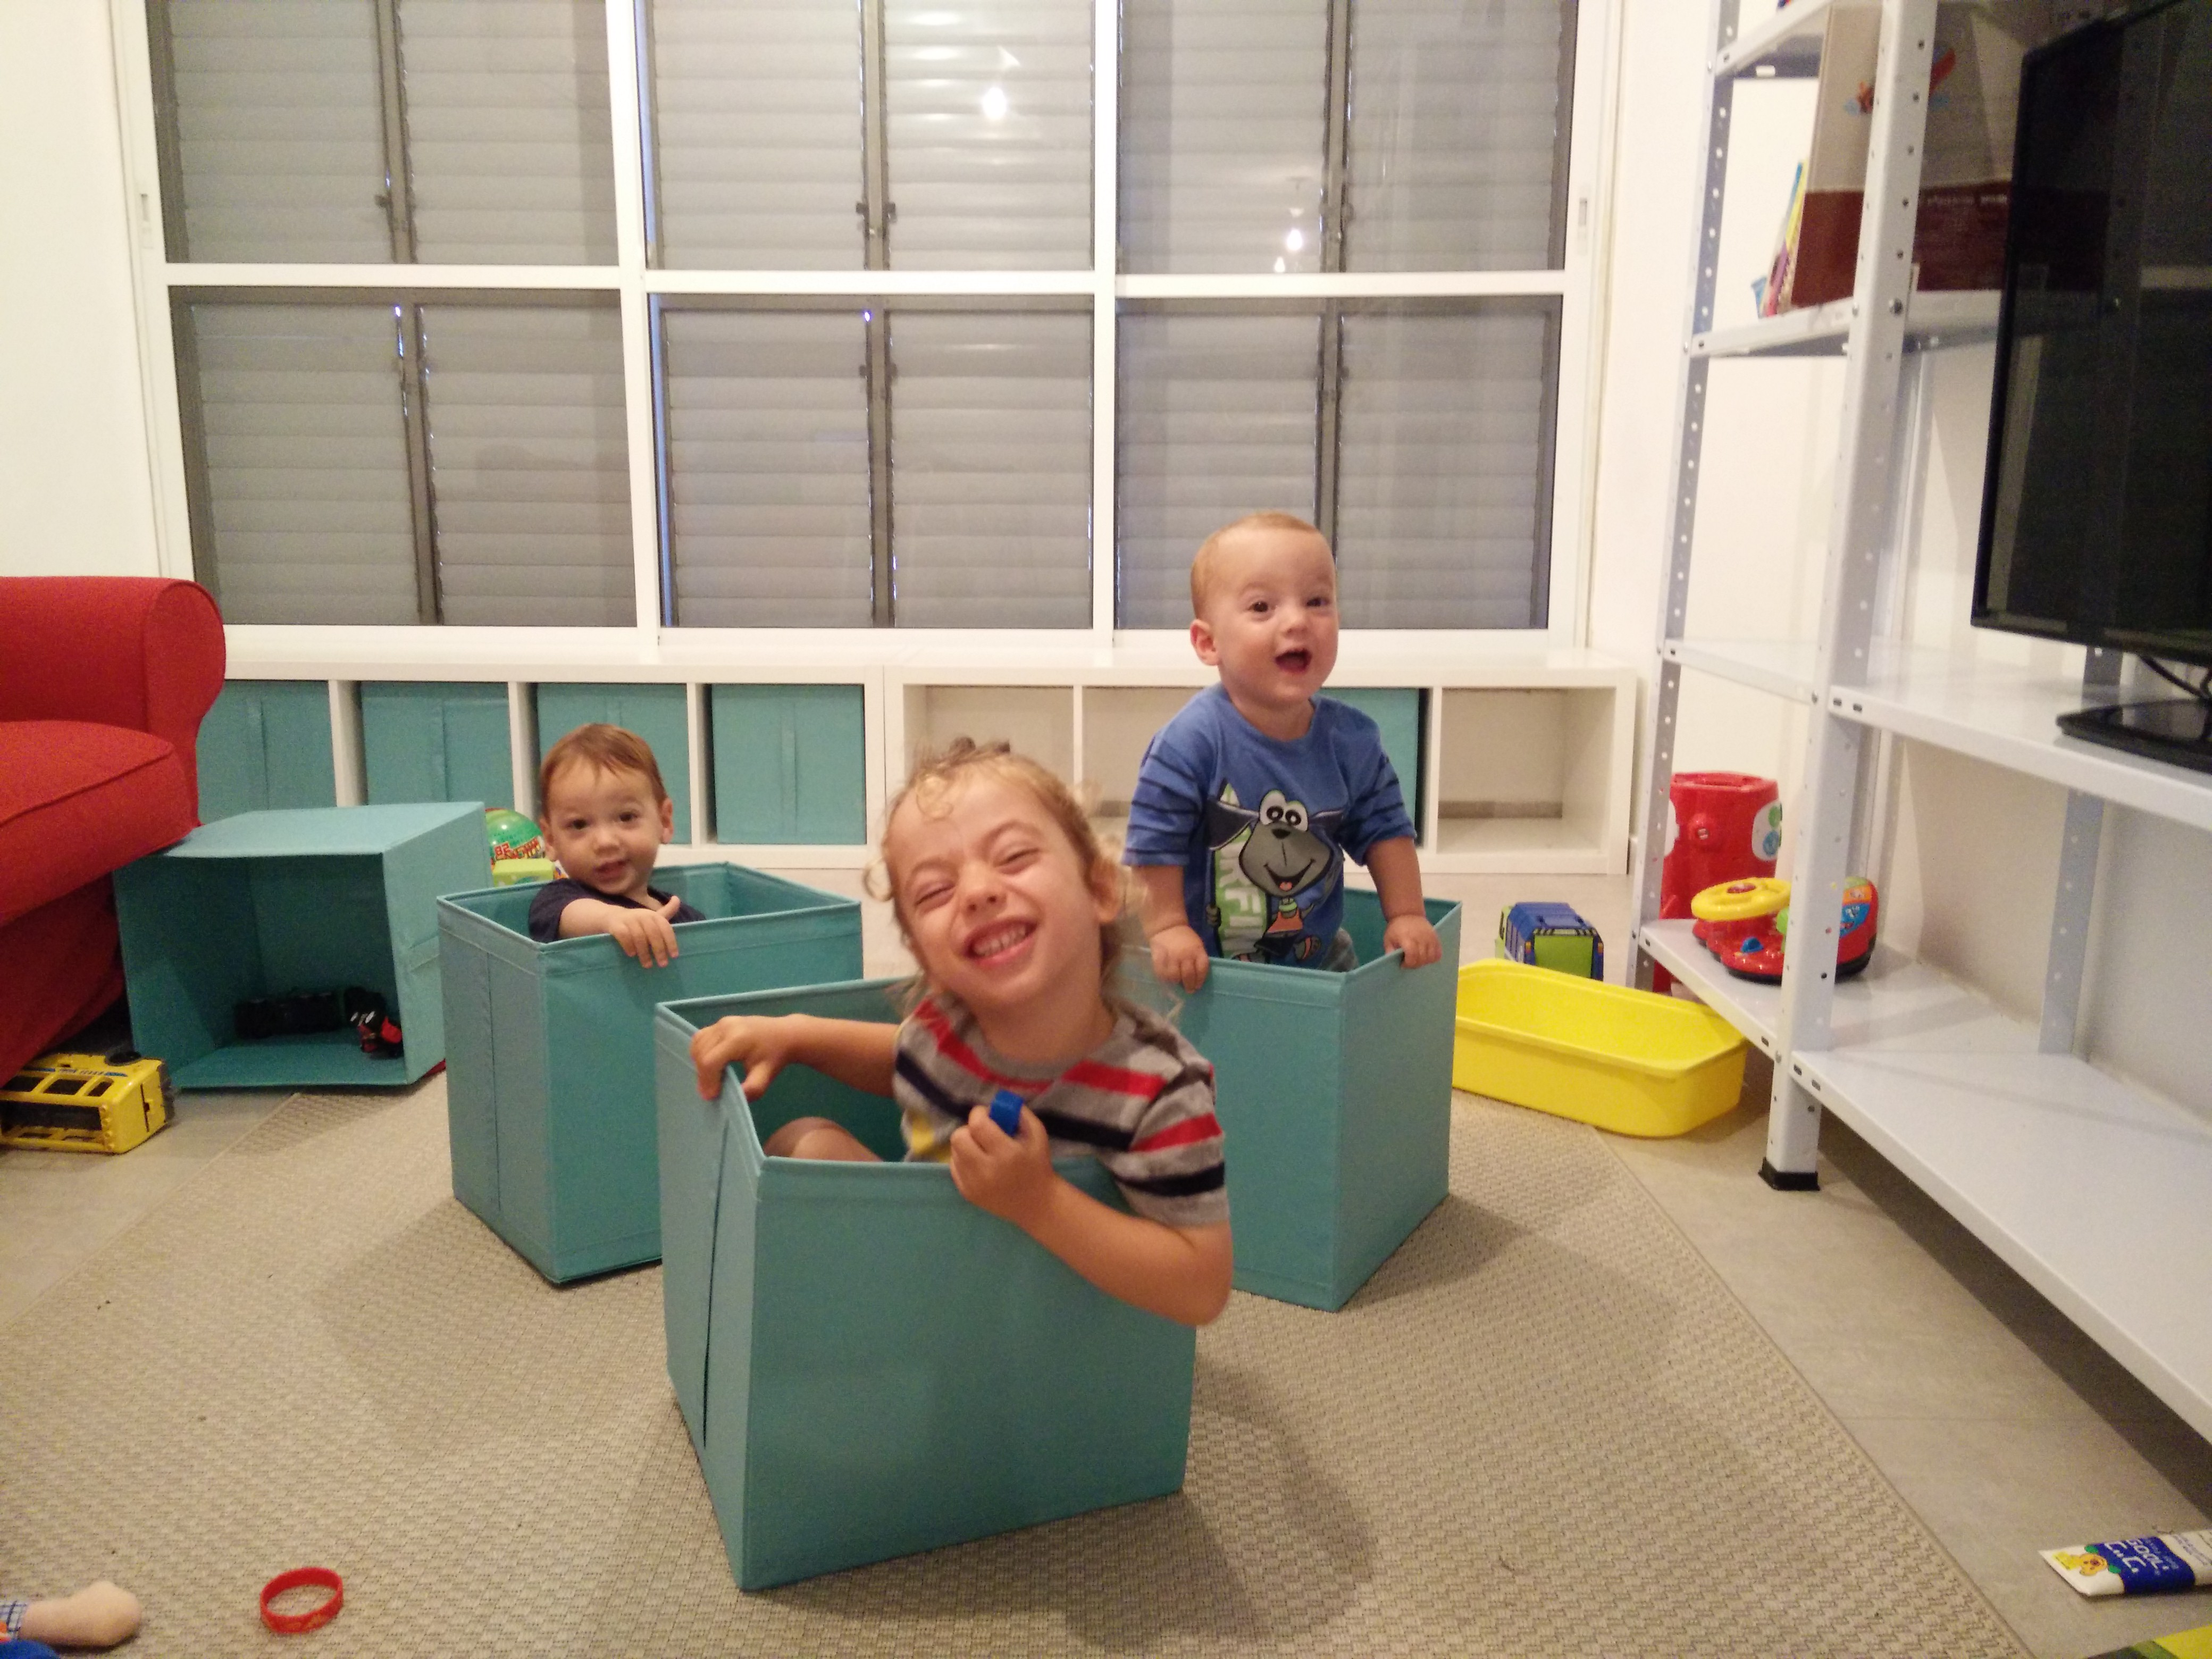
\includegraphics[width=0.3\textwidth]{pictures/boys.jpg}
    \end{center}
\vfill
  
\end{frame}  

\begin{frame}
  \frametitle{Acknowledgments}

  \begin{center}
    \Huge Thank You!
  \end{center}
  \bibliographystyle{plain}
  \nobibliography{mybib}
\end{frame}

% \input{sections/Appendix.tex}
\end{document}
